% Options for packages loaded elsewhere
% Options for packages loaded elsewhere
\PassOptionsToPackage{unicode}{hyperref}
\PassOptionsToPackage{hyphens}{url}
\PassOptionsToPackage{dvipsnames,svgnames,x11names}{xcolor}
%
\documentclass[
  letterpaper,
]{scrbook}
\usepackage{xcolor}
\usepackage[margin=1in]{geometry}
\usepackage{amsmath,amssymb}
\setcounter{secnumdepth}{3}
\usepackage{iftex}
\ifPDFTeX
  \usepackage[T1]{fontenc}
  \usepackage[utf8]{inputenc}
  \usepackage{textcomp} % provide euro and other symbols
\else % if luatex or xetex
  \usepackage{unicode-math} % this also loads fontspec
  \defaultfontfeatures{Scale=MatchLowercase}
  \defaultfontfeatures[\rmfamily]{Ligatures=TeX,Scale=1}
\fi
\usepackage{lmodern}
\ifPDFTeX\else
  % xetex/luatex font selection
\fi
% Use upquote if available, for straight quotes in verbatim environments
\IfFileExists{upquote.sty}{\usepackage{upquote}}{}
\IfFileExists{microtype.sty}{% use microtype if available
  \usepackage[]{microtype}
  \UseMicrotypeSet[protrusion]{basicmath} % disable protrusion for tt fonts
}{}
\makeatletter
\@ifundefined{KOMAClassName}{% if non-KOMA class
  \IfFileExists{parskip.sty}{%
    \usepackage{parskip}
  }{% else
    \setlength{\parindent}{0pt}
    \setlength{\parskip}{6pt plus 2pt minus 1pt}}
}{% if KOMA class
  \KOMAoptions{parskip=half}}
\makeatother
% Make \paragraph and \subparagraph free-standing
\makeatletter
\ifx\paragraph\undefined\else
  \let\oldparagraph\paragraph
  \renewcommand{\paragraph}{
    \@ifstar
      \xxxParagraphStar
      \xxxParagraphNoStar
  }
  \newcommand{\xxxParagraphStar}[1]{\oldparagraph*{#1}\mbox{}}
  \newcommand{\xxxParagraphNoStar}[1]{\oldparagraph{#1}\mbox{}}
\fi
\ifx\subparagraph\undefined\else
  \let\oldsubparagraph\subparagraph
  \renewcommand{\subparagraph}{
    \@ifstar
      \xxxSubParagraphStar
      \xxxSubParagraphNoStar
  }
  \newcommand{\xxxSubParagraphStar}[1]{\oldsubparagraph*{#1}\mbox{}}
  \newcommand{\xxxSubParagraphNoStar}[1]{\oldsubparagraph{#1}\mbox{}}
\fi
\makeatother


\usepackage{longtable,booktabs,array}
\usepackage{calc} % for calculating minipage widths
% Correct order of tables after \paragraph or \subparagraph
\usepackage{etoolbox}
\makeatletter
\patchcmd\longtable{\par}{\if@noskipsec\mbox{}\fi\par}{}{}
\makeatother
% Allow footnotes in longtable head/foot
\IfFileExists{footnotehyper.sty}{\usepackage{footnotehyper}}{\usepackage{footnote}}
\makesavenoteenv{longtable}
\usepackage{graphicx}
\makeatletter
\newsavebox\pandoc@box
\newcommand*\pandocbounded[1]{% scales image to fit in text height/width
  \sbox\pandoc@box{#1}%
  \Gscale@div\@tempa{\textheight}{\dimexpr\ht\pandoc@box+\dp\pandoc@box\relax}%
  \Gscale@div\@tempb{\linewidth}{\wd\pandoc@box}%
  \ifdim\@tempb\p@<\@tempa\p@\let\@tempa\@tempb\fi% select the smaller of both
  \ifdim\@tempa\p@<\p@\scalebox{\@tempa}{\usebox\pandoc@box}%
  \else\usebox{\pandoc@box}%
  \fi%
}
% Set default figure placement to htbp
\def\fps@figure{htbp}
\makeatother


% definitions for citeproc citations
\NewDocumentCommand\citeproctext{}{}
\NewDocumentCommand\citeproc{mm}{%
  \begingroup\def\citeproctext{#2}\cite{#1}\endgroup}
\makeatletter
 % allow citations to break across lines
 \let\@cite@ofmt\@firstofone
 % avoid brackets around text for \cite:
 \def\@biblabel#1{}
 \def\@cite#1#2{{#1\if@tempswa , #2\fi}}
\makeatother
\newlength{\cslhangindent}
\setlength{\cslhangindent}{1.5em}
\newlength{\csllabelwidth}
\setlength{\csllabelwidth}{3em}
\newenvironment{CSLReferences}[2] % #1 hanging-indent, #2 entry-spacing
 {\begin{list}{}{%
  \setlength{\itemindent}{0pt}
  \setlength{\leftmargin}{0pt}
  \setlength{\parsep}{0pt}
  % turn on hanging indent if param 1 is 1
  \ifodd #1
   \setlength{\leftmargin}{\cslhangindent}
   \setlength{\itemindent}{-1\cslhangindent}
  \fi
  % set entry spacing
  \setlength{\itemsep}{#2\baselineskip}}}
 {\end{list}}
\usepackage{calc}
\newcommand{\CSLBlock}[1]{\hfill\break\parbox[t]{\linewidth}{\strut\ignorespaces#1\strut}}
\newcommand{\CSLLeftMargin}[1]{\parbox[t]{\csllabelwidth}{\strut#1\strut}}
\newcommand{\CSLRightInline}[1]{\parbox[t]{\linewidth - \csllabelwidth}{\strut#1\strut}}
\newcommand{\CSLIndent}[1]{\hspace{\cslhangindent}#1}



\setlength{\emergencystretch}{3em} % prevent overfull lines

\providecommand{\tightlist}{%
  \setlength{\itemsep}{0pt}\setlength{\parskip}{0pt}}



 


\usepackage{fancyhdr}

% Header / footer style
\pagestyle{fancy}
\fancyhead[L]{FastMAPOL ATBD}
\fancyhead[R]{Draft}
\fancyfoot[C]{\thepage}

% Rename Appendix (KOMA-compatible)
\renewcommand{\appendixname}{Technical Details}
\makeatletter
\@ifpackageloaded{bookmark}{}{\usepackage{bookmark}}
\makeatother
\makeatletter
\@ifpackageloaded{caption}{}{\usepackage{caption}}
\AtBeginDocument{%
\ifdefined\contentsname
  \renewcommand*\contentsname{Table of contents}
\else
  \newcommand\contentsname{Table of contents}
\fi
\ifdefined\listfigurename
  \renewcommand*\listfigurename{List of Figures}
\else
  \newcommand\listfigurename{List of Figures}
\fi
\ifdefined\listtablename
  \renewcommand*\listtablename{List of Tables}
\else
  \newcommand\listtablename{List of Tables}
\fi
\ifdefined\figurename
  \renewcommand*\figurename{Figure}
\else
  \newcommand\figurename{Figure}
\fi
\ifdefined\tablename
  \renewcommand*\tablename{Table}
\else
  \newcommand\tablename{Table}
\fi
}
\@ifpackageloaded{float}{}{\usepackage{float}}
\floatstyle{ruled}
\@ifundefined{c@chapter}{\newfloat{codelisting}{h}{lop}}{\newfloat{codelisting}{h}{lop}[chapter]}
\floatname{codelisting}{Listing}
\newcommand*\listoflistings{\listof{codelisting}{List of Listings}}
\makeatother
\makeatletter
\makeatother
\makeatletter
\@ifpackageloaded{caption}{}{\usepackage{caption}}
\@ifpackageloaded{subcaption}{}{\usepackage{subcaption}}
\makeatother
\usepackage{bookmark}
\IfFileExists{xurl.sty}{\usepackage{xurl}}{} % add URL line breaks if available
\urlstyle{same}
\hypersetup{
  pdftitle={FastMAPOL Algorithm Theoretical Basis Document},
  pdfauthor={Drafting},
  colorlinks=true,
  linkcolor={Maroon},
  filecolor={Maroon},
  citecolor={Blue},
  urlcolor={Blue},
  pdfcreator={LaTeX via pandoc}}


\title{FastMAPOL Algorithm Theoretical Basis Document}
\usepackage{etoolbox}
\makeatletter
\providecommand{\subtitle}[1]{% add subtitle to \maketitle
  \apptocmd{\@title}{\par {\large #1 \par}}{}{}
}
\makeatother
\subtitle{PACE Polarimeter Aerosol and Ocean Retrieval}
\author{Drafting}
\date{2026-03-26}
\begin{document}
\frontmatter
\maketitle

\renewcommand*\contentsname{Table of contents}
{
\hypersetup{linkcolor=}
\setcounter{tocdepth}{2}
\tableofcontents
}
\listoffigures
\listoftables

\mainmatter
\bookmarksetup{startatroot}

\chapter{FastMAPOL Algorithm Theoretical Basis
Document}\label{fastmapol-algorithm-theoretical-basis-document}

PACE Multi-Angle Polarimetric Aerosol and Ocean Retrieval

\hfill\break

\bookmarksetup{startatroot}

\chapter{Executive Summary}\label{executive-summary}

FastMAPOL (Fast Multi-Angle Polarimetric Ocean and Land) is a nonlinear
least-squares retrieval algorithm developed for the NASA PACE mission.
It retrieves aerosol and ocean optical properties from multi-angle
polarimetric observations acquired by the PACE polarimeters, including
HARP2 and SPEXone.

The algorithm uses neural networks to emulate polarized radiative
transfer, significantly improving computational efficiency and enabling
operational-scale processing. FastMAPOL produces a comprehensive suite
of environmental data records along with associated uncertainty
estimates. Main features include: - Coupled Atmosphere-surface radiaitve
transfer model (PACE-Simulator) - Cascaed neural network emulator, and
analytical Jacobians - Optimal estimation based on non-linear least
square minimzation - Adaptive data screening - Pixel-level uncertainty
estimation - Uncertainty correlation

Retrieval products include aersol optical, microphysical properties,
multi-angle ocean color products, etc

This document describes the theoretical framework, forward modeling,
inversion methodology, and data products generated by FastMAPOL.

\begin{center}\rule{0.5\linewidth}{0.5pt}\end{center}

\bookmarksetup{startatroot}

\chapter{Introduction}\label{introduction}

The PACE mission includes three instruments:

\begin{itemize}
\tightlist
\item
  Ocean Color Instrument (OCI)\\
\item
  Hyper-Angular Rainbow Polarimeter-2 (HARP2)\\
\item
  SPEXone polarimeter
\end{itemize}

Multi-angle polarimetric observations provide enhanced sensitivity to
aerosol microphysical properties and ocean optical parameters. FastMAPOL
is designed to exploit this information content through a physics-based
inversion framework accelerated by machine learning.

\begin{center}\rule{0.5\linewidth}{0.5pt}\end{center}

\bookmarksetup{startatroot}

\chapter{Scope of Document}\label{scope-of-document}

This Algorithm Theoretical Basis Document (ATBD) describes the
methodology used in FastMAPOL to retrieve aerosol and ocean properties
from PACE polarimeter measurements.

The document includes the following components:

\begin{itemize}
\tightlist
\item
  Algorithm architecture and components\\
\item
  Aerosol optical model\\
\item
  Ocean bio-optical model\\
\item
  Land surface model\\
\item
  Neural network forward model\\
\item
  Retrieval methodology and uncertainty quantification\\
\item
  Level-2 data product definition\\
\item
  Validation using HARP2 and SPEXone observations
\end{itemize}

\begin{center}\rule{0.5\linewidth}{0.5pt}\end{center}

\bookmarksetup{startatroot}

\chapter{Document Organization}\label{document-organization}

The remainder of this document is organized as follows: - main chapters
describe major algorithm components, data product format and validations
- Appendices provide additional technical details

\begin{center}\rule{0.5\linewidth}{0.5pt}\end{center}

\bookmarksetup{startatroot}

\chapter{Document Information}\label{document-information}

\begin{longtable}[]{@{}ll@{}}
\toprule\noalign{}
Item & Description \\
\midrule\noalign{}
\endhead
\bottomrule\noalign{}
\endlastfoot
Document Title & FastMAPOL Algorithm Theoretical Basis Document \\
Version & Draft \\
Date & 2026 \\
Authors & Meng Gao et al. \\
Institution & NASA GSFC \\
Project & PACE Mission \\
\end{longtable}

\begin{center}\rule{0.5\linewidth}{0.5pt}\end{center}

\bookmarksetup{startatroot}

\chapter{FastMAPOL in a nutshell}\label{fastmapol-in-a-nutshell}

before reading the full document, this chaper provide high level summary
of the algorithm, product, format and validations.

details will be in each chapter

Major features

\begin{itemize}
\tightlist
\item
  Flexible vector radiative transfer
\item
  NN forward model
\item
  NN Jacobian
\item
  Adaptive data screening
\item
  Pixelwise uncertainty estimation
\item
  Uncertainty correlation
\item
  Coupled atmosphere and surface product
\item
  Uncertainty closure
\item
  BRDF closure
\end{itemize}

\bookmarksetup{startatroot}

\chapter{Retrieval algorithm}\label{retrieval-algorithm}

\section{Cost function}\label{cost-function}

Chi2 function Chi2 statistics \#\# Uncertaint model forward model
numerical accuracy, NN accuracy, measurement uncertainty \#\# Iversion
Optimization

\section{STIR}\label{stir}

\bookmarksetup{startatroot}

\chapter{Neural network forward model and Analytical
Jacobian}\label{neural-network-forward-model-and-analytical-jacobian}

\section{Neural network forward
model}\label{neural-network-forward-model}

\section{NN training}\label{nn-training}

\section{NN uncertainty}\label{nn-uncertainty}

\section{Analytical Jacobians}\label{analytical-jacobians}

\bookmarksetup{startatroot}

\chapter{Radiative transfer model for PACE (PACE
Simulator)}\label{radiative-transfer-model-for-pace-pace-simulator}

The Radiative Transfer model is based on the Successive Order of
Scattering (RTSOS) method (Zhai et al., 2009, 2010).

Key features: - RTSOS is capable of solving polarized radiative transfer
for both atmosphere-ocean and atmosphere-land systems. - In
atmosphere-ocean systems, it can also simulate inelastic scattering
processes, including Raman scattering and fluorescence by chlorophyll
and colored dissolved organic matter (Zhai et al., 2015, 2017, 2018). -
An improved pseudos-spherical shell (IPSS) algorithm is used to improve
the simulation of radiance field over polar regions (Zhai and Hu, 2022).

For this work, RTSOS is configured to simulate polarized radiance fields
for randomly generated Earth systems for the PACE instruments (Zhai et
al, 2022). The data are then used to train neural network forward
models, which emulates the behavior of the radiative transfer system.

\section{Code repository}\label{code-repository}

The RTSOS is made public by Dr.~Pengwang Zhai in github (\ldots)

\bookmarksetup{startatroot}

\chapter{}\label{section}

\bookmarksetup{startatroot}

\chapter{Multi-angle ocean color
product}\label{multi-angle-ocean-color-product}

\section{Atmospheric correction}\label{atmospheric-correction}

\section{BRDF correction}\label{brdf-correction}

\bookmarksetup{startatroot}

\chapter{Data Products and Format}\label{data-products-and-format}

\section{Overview}\label{overview}

FastMAPOL (Fast Multi-Angle Polarimetric Ocean and Land algorithm)
produces Level-2 (L2) geophysical retrievals of aerosol and surface
properties from the multi-angle polarimetric measurements of the
\textbf{PACE polarimeters}, including \textbf{HARP2} and
\textbf{SPEXone}.

The Level-2 product provides pixel-level estimates of aerosol optical
properties, aerosol microphysical parameters, and ocean color quantities
derived through atmospheric correction. In addition to the primary
geophysical retrievals, the product includes diagnostic quantities
describing retrieval performance and quality indicators for downstream
processing.

The Level-2 product is distributed in \textbf{NetCDF format} and
organized into hierarchical data groups to separate geolocation,
geophysical variables, diagnostics, and sensor parameters.

The FastMAPOL Level-2 product is designed to support:

\begin{itemize}
\tightlist
\item
  aerosol science applications
\item
  ocean color retrievals
\item
  atmospheric correction
\item
  algorithm validation
\item
  Level-3 gridded product generation
\end{itemize}

\begin{center}\rule{0.5\linewidth}{0.5pt}\end{center}

\section{File Organization}\label{file-organization}

The FastMAPOL Level-2 file is organized into several top-level groups.
Each group contains variables associated with a specific component of
the retrieval system.

\begin{longtable}[]{@{}ll@{}}
\toprule\noalign{}
Group & Description \\
\midrule\noalign{}
\endhead
\bottomrule\noalign{}
\endlastfoot
geolocation\_data & Pixel geolocation information \\
geophysical\_data & Primary aerosol and ocean retrieval products \\
diagnostic\_data & Retrieval diagnostics and performance metrics \\
sensor\_band\_parameters & Instrument spectral and angular parameters \\
processing\_control & Metadata and algorithm configuration \\
\end{longtable}

\subsection{Dimensions}\label{dimensions}

The FastMAPOL Level-2 product uses a set of core dimensions describing
spatial, spectral, and angular sampling.

\begin{longtable}[]{@{}ll@{}}
\toprule\noalign{}
Dimension & Description \\
\midrule\noalign{}
\endhead
\bottomrule\noalign{}
\endlastfoot
number\_of\_lines & Number of along-track scan lines \\
pixels\_per\_line & Number of cross-track pixels \\
wavelength & Spectral bands used in retrieval \\
number\_of\_views & Viewing angles used in the retrieval \\
intensity\_bands\_per\_view & Intensity channels per view \\
polarization\_bands\_per\_view & Polarization channels per view \\
\end{longtable}

\subsection{Instrument Differences}\label{instrument-differences}

\textbf{HARP2}

\begin{itemize}
\tightlist
\item
  \textasciitilde90 viewing angles\\
\item
  4 spectral bands : 440, 550, 670, 870nm
\item
  wide swath (\textasciitilde2000km)
\end{itemize}

\textbf{SPEXone}

\begin{itemize}
\tightlist
\item
  5 viewing angles\\
\item
  hyperspectral polarimetric measurements 50
\item
  narrow swath (\textasciitilde100km)
\end{itemize}

A total of 34 specific wavelengths from the hyperspectral measurements
for aerosol and surface retrieval.

\section{Geolocation Data}\label{geolocation-data}

Group: \texttt{/geolocation\_data}

\begin{longtable}[]{@{}lll@{}}
\toprule\noalign{}
Variable & Dimensions & Description \\
\midrule\noalign{}
\endhead
\bottomrule\noalign{}
\endlastfoot
latitude & (number\_of\_lines, pixels\_per\_line) & Pixel latitude \\
longitude & (number\_of\_lines, pixels\_per\_line) & Pixel longitude \\
\end{longtable}

These variables define the geographic location of each retrieval pixel.

\section{Geophysical Retrieval
Products}\label{geophysical-retrieval-products}

Group: \texttt{/geophysical\_data}

The geophysical group contains aerosol optical properties, aerosol
microphysical parameters, and ocean color products retrieved by
FastMAPOL.

\subsection{Aerosol Optical
Properties}\label{aerosol-optical-properties}

\begin{longtable}[]{@{}
  >{\raggedright\arraybackslash}p{(\linewidth - 4\tabcolsep) * \real{0.2778}}
  >{\raggedright\arraybackslash}p{(\linewidth - 4\tabcolsep) * \real{0.3611}}
  >{\raggedright\arraybackslash}p{(\linewidth - 4\tabcolsep) * \real{0.3611}}@{}}
\toprule\noalign{}
\begin{minipage}[b]{\linewidth}\raggedright
Variable
\end{minipage} & \begin{minipage}[b]{\linewidth}\raggedright
Dimensions
\end{minipage} & \begin{minipage}[b]{\linewidth}\raggedright
Description
\end{minipage} \\
\midrule\noalign{}
\endhead
\bottomrule\noalign{}
\endlastfoot
aot & (number\_of\_lines, pixels\_per\_line, wavelength) & Aerosol
optical depth \\
aot\_fine & (number\_of\_lines, pixels\_per\_line, wavelength) &
Fine-mode optical depth \\
aot\_coarse & (number\_of\_lines, pixels\_per\_line, wavelength) &
Coarse-mode optical depth \\
ssa & (number\_of\_lines, pixels\_per\_line, wavelength) & Aerosol
single scattering albedo \\
ssa\_fine & (number\_of\_lines, pixels\_per\_line, wavelength) &
Fine-mode SSA \\
ssa\_coarse & (number\_of\_lines, pixels\_per\_line, wavelength) &
Coarse-mode SSA \\
angstrom\_440\_870 & (number\_of\_lines, pixels\_per\_line) & Ångström
exponent (440-870 nm) \\
angstrom\_440\_670 & (number\_of\_lines, pixels\_per\_line) & Ångström
exponent (440-670 nm) \\
fmf & (number\_of\_lines, pixels\_per\_line) & Fine-mode optical depth
fraction \\
\end{longtable}

These parameters describe aerosol optical loading and spectral behavior.

\subsection{Aerosol Microphysical
Properties}\label{aerosol-microphysical-properties}

\begin{longtable}[]{@{}
  >{\raggedright\arraybackslash}p{(\linewidth - 4\tabcolsep) * \real{0.2778}}
  >{\raggedright\arraybackslash}p{(\linewidth - 4\tabcolsep) * \real{0.3611}}
  >{\raggedright\arraybackslash}p{(\linewidth - 4\tabcolsep) * \real{0.3611}}@{}}
\toprule\noalign{}
\begin{minipage}[b]{\linewidth}\raggedright
Variable
\end{minipage} & \begin{minipage}[b]{\linewidth}\raggedright
Dimensions
\end{minipage} & \begin{minipage}[b]{\linewidth}\raggedright
Description
\end{minipage} \\
\midrule\noalign{}
\endhead
\bottomrule\noalign{}
\endlastfoot
reff\_fine & (number\_of\_lines, pixels\_per\_line) & Fine-mode
effective radius \\
reff\_coarse & (number\_of\_lines, pixels\_per\_line) & Coarse-mode
effective radius \\
veff\_fine & (number\_of\_lines, pixels\_per\_line) & Fine-mode
effective variance \\
veff\_coarse & (number\_of\_lines, pixels\_per\_line) & Coarse-mode
effective variance \\
mr & (number\_of\_lines, pixels\_per\_line, wavelength) & Real
refractive index \\
mi & (number\_of\_lines, pixels\_per\_line, wavelength) & Imaginary
refractive index \\
sph & (number\_of\_lines, pixels\_per\_line) & Spherical particle
fraction \\
vd\_fine & (number\_of\_lines, pixels\_per\_line) & Fine-mode volume
density \\
vd\_coarse & (number\_of\_lines, pixels\_per\_line) & Coarse-mode volume
density \\
fvf & (number\_of\_lines, pixels\_per\_line) & Fine-mode volume
fraction \\
alh & (number\_of\_lines, pixels\_per\_line) & Aerosol layer height \\
\end{longtable}

These variables constrain aerosol particle size distribution,
composition, and shape.

\subsection{Ocean Color Products}\label{ocean-color-products}

\begin{longtable}[]{@{}
  >{\raggedright\arraybackslash}p{(\linewidth - 4\tabcolsep) * \real{0.2778}}
  >{\raggedright\arraybackslash}p{(\linewidth - 4\tabcolsep) * \real{0.3611}}
  >{\raggedright\arraybackslash}p{(\linewidth - 4\tabcolsep) * \real{0.3611}}@{}}
\toprule\noalign{}
\begin{minipage}[b]{\linewidth}\raggedright
Variable
\end{minipage} & \begin{minipage}[b]{\linewidth}\raggedright
Dimensions
\end{minipage} & \begin{minipage}[b]{\linewidth}\raggedright
Description
\end{minipage} \\
\midrule\noalign{}
\endhead
\bottomrule\noalign{}
\endlastfoot
Rrs1 & (number\_of\_lines, pixels\_per\_line, wavelength,
number\_of\_views) & Remote sensing reflectance before BRDF
correction \\
Rrs2 & (number\_of\_lines, pixels\_per\_line, wavelength,
number\_of\_views) & Remote sensing reflectance after BRDF correction \\
Rrs1\_mean & (number\_of\_lines, pixels\_per\_line, wavelength) &
Angular mean of Rrs1 \\
Rrs1\_std & (number\_of\_lines, pixels\_per\_line, wavelength) & Angular
standard deviation of Rrs1 \\
Rrs2\_mean & (number\_of\_lines, pixels\_per\_line, wavelength) &
Angular mean of Rrs2 \\
Rrs2\_std & (number\_of\_lines, pixels\_per\_line, wavelength) & Angular
standard deviation of Rrs2 \\
\end{longtable}

The remote sensing reflectance represents ocean-leaving reflectance
after atmospheric correction.

Because the full angular arrays can be large, the Level-2 product
typically includes the \textbf{angular mean and standard deviation}.

\subsection{Additional Surface
Variables}\label{additional-surface-variables}

\begin{longtable}[]{@{}
  >{\raggedright\arraybackslash}p{(\linewidth - 4\tabcolsep) * \real{0.2778}}
  >{\raggedright\arraybackslash}p{(\linewidth - 4\tabcolsep) * \real{0.3611}}
  >{\raggedright\arraybackslash}p{(\linewidth - 4\tabcolsep) * \real{0.3611}}@{}}
\toprule\noalign{}
\begin{minipage}[b]{\linewidth}\raggedright
Variable
\end{minipage} & \begin{minipage}[b]{\linewidth}\raggedright
Dimensions
\end{minipage} & \begin{minipage}[b]{\linewidth}\raggedright
Description
\end{minipage} \\
\midrule\noalign{}
\endhead
\bottomrule\noalign{}
\endlastfoot
wind\_speed & (number\_of\_lines, pixels\_per\_line) & Surface wind
speed \\
chla & (number\_of\_lines, pixels\_per\_line) & Chlorophyll-a
concentration \\
\end{longtable}

\section{Diagnostic Data}\label{diagnostic-data}

Group: \texttt{/diagnostic\_data}

These variables describe retrieval convergence and performance.

\begin{longtable}[]{@{}
  >{\raggedright\arraybackslash}p{(\linewidth - 4\tabcolsep) * \real{0.2778}}
  >{\raggedright\arraybackslash}p{(\linewidth - 4\tabcolsep) * \real{0.3611}}
  >{\raggedright\arraybackslash}p{(\linewidth - 4\tabcolsep) * \real{0.3611}}@{}}
\toprule\noalign{}
\begin{minipage}[b]{\linewidth}\raggedright
Variable
\end{minipage} & \begin{minipage}[b]{\linewidth}\raggedright
Dimensions
\end{minipage} & \begin{minipage}[b]{\linewidth}\raggedright
Description
\end{minipage} \\
\midrule\noalign{}
\endhead
\bottomrule\noalign{}
\endlastfoot
chi2 & (number\_of\_lines, pixels\_per\_line) & Retrieval cost
function \\
chi2\_first\_guess & (number\_of\_lines, pixels\_per\_line) & Cost
function at first guess \\
nv\_ref & (number\_of\_lines, pixels\_per\_line) & Number of reflectance
measurements used \\
nv\_dolp & (number\_of\_lines, pixels\_per\_line) & Number of
polarization measurements used \\
nfev & (number\_of\_lines, pixels\_per\_line) & Number of forward model
evaluations \\
njev & (number\_of\_lines, pixels\_per\_line) & Number of Jacobian
evaluations \\
timing & (number\_of\_lines, pixels\_per\_line) & Retrieval runtime \\
quality\_flag & (number\_of\_lines, pixels\_per\_line) & Retrieval
quality indicator \\
ozone & (number\_of\_lines, pixels\_per\_line) & Total column ozone \\
surface\_pressure & (number\_of\_lines, pixels\_per\_line) & Surface
pressure \\
\end{longtable}

\subsection{Retrieval Quality Metrics}\label{retrieval-quality-metrics}

FastMAPOL retrievals are performed using an optimal estimation framework
that minimizes the cost function

\[
\chi^2 = \frac{1}{N}\sum \frac{(f-m)^2}{\sigma^2}
\]

where

\begin{itemize}
\tightlist
\item
  \(m\) is the measurement\\
\item
  \(f\) is the forward model simulation
\item
  \(\sigma\) is measurement uncertainty\\
\item
  \(N\) is the number of measurements used in the retrieval.
\end{itemize}

Lower values of \(\chi^2\) indicate better agreement between
measurements and forward model simulations.

\subsection{Retrieval Quality Flag}\label{retrieval-quality-flag}

A quality flag is provided to facilitate filtering and Level-3
processing.

\begin{longtable}[]{@{}ll@{}}
\toprule\noalign{}
quality\_flag & Description \\
\midrule\noalign{}
\endhead
\bottomrule\noalign{}
\endlastfoot
0 & highest retrieval quality \\
1 & good retrieval quality \\
\textgreater1 & reduced quality \\
\end{longtable}

The quality flag is determined from combinations of:

\begin{itemize}
\tightlist
\item
  cost function value
\item
  number of reflectance measurements
\item
  number of polarization measurements.
\end{itemize}

\subsection{Measurement Screening
Masks}\label{measurement-screening-masks}

FastMAPOL performs adaptive measurement screening during the inversion.

\begin{longtable}[]{@{}
  >{\raggedright\arraybackslash}p{(\linewidth - 4\tabcolsep) * \real{0.2778}}
  >{\raggedright\arraybackslash}p{(\linewidth - 4\tabcolsep) * \real{0.3611}}
  >{\raggedright\arraybackslash}p{(\linewidth - 4\tabcolsep) * \real{0.3611}}@{}}
\toprule\noalign{}
\begin{minipage}[b]{\linewidth}\raggedright
Variable
\end{minipage} & \begin{minipage}[b]{\linewidth}\raggedright
Dimensions
\end{minipage} & \begin{minipage}[b]{\linewidth}\raggedright
Description
\end{minipage} \\
\midrule\noalign{}
\endhead
\bottomrule\noalign{}
\endlastfoot
mask\_ref & (number\_of\_lines, pixels\_per\_line, number\_of\_views,
intensity\_bands\_per\_view) & Reflectance measurement mask \\
mask\_dolp & (number\_of\_lines, pixels\_per\_line, number\_of\_views,
polarization\_bands\_per\_view) & Polarization measurement mask \\
\end{longtable}

Mask interpretation:

\begin{longtable}[]{@{}ll@{}}
\toprule\noalign{}
Value & Meaning \\
\midrule\noalign{}
\endhead
\bottomrule\noalign{}
\endlastfoot
0 & measurement used in retrieval \\
1 or NaN & measurement excluded from retrieval \\
\end{longtable}

These masks allow users to evaluate measurement quality at each viewing
angle.

\section{Sensor Band Parameters}\label{sensor-band-parameters}

Group: \texttt{/sensor\_band\_parameters}

\begin{longtable}[]{@{}lll@{}}
\toprule\noalign{}
Variable & Dimensions & Description \\
\midrule\noalign{}
\endhead
\bottomrule\noalign{}
\endlastfoot
wavelength & (wavelength) & Retrieval wavelengths \\
sensor\_view\_angle & (number\_of\_views) & Viewing angle geometry \\
\end{longtable}

\bookmarksetup{startatroot}

\chapter{HARP2 L2 aerosol product validation (Pre-Launch DITL
test)}\label{harp2-l2-aerosol-product-validation-pre-launch-ditl-test}

\section{Overview}\label{overview-1}

Pre-launch Day-in-the-Life (DITL) simulations provide an end-to-end
benchmark of HARP2 measurement realism, L2 retrieval performance, and
uncertainty characterization. The results below highlight three key
aspects: synthetic observations, pixel-wise retrieval performance, and
uncertainty analysis. Details are provided in M. Gao et al. (2023).

\section{Summary Information}\label{summary-information}

\begin{itemize}
\tightlist
\item
  \textbf{FastMAPOL version:} Prelaunch Test\\
\item
  \textbf{Data period:} March 21, 2022 (spring equinox)\\
\item
  \textbf{Reference:} Synthetic HARP2\\
\item
  \textbf{Published:} Dec 07, 2023
  (https://doi.org/10.5194/amt-16-5863-2023)
\end{itemize}

\section{Synthetic HARP2
observations}\label{synthetic-harp2-observations}

As shown in Figure~\ref{fig-validation_harp2_l1c}, A full day of
synthetic HARP2 observations is generated using a neural network forward
model for both reflectance and DoLP. Aerosol and surface properties are
prescribed from reanalysis (MERRA-2). The simulated observations provide
a realistic testbed for retrieval evaluation:

\begin{itemize}
\tightlist
\item
  Global multi-angle measurements are generated for both reflectance and
  polarization.\\
\item
  DoLP shows enhanced sensitivity to aerosol and surface properties.\\
\item
  Reflectance and DoLP provide complementary information content.
\end{itemize}

\begin{figure}

\centering{

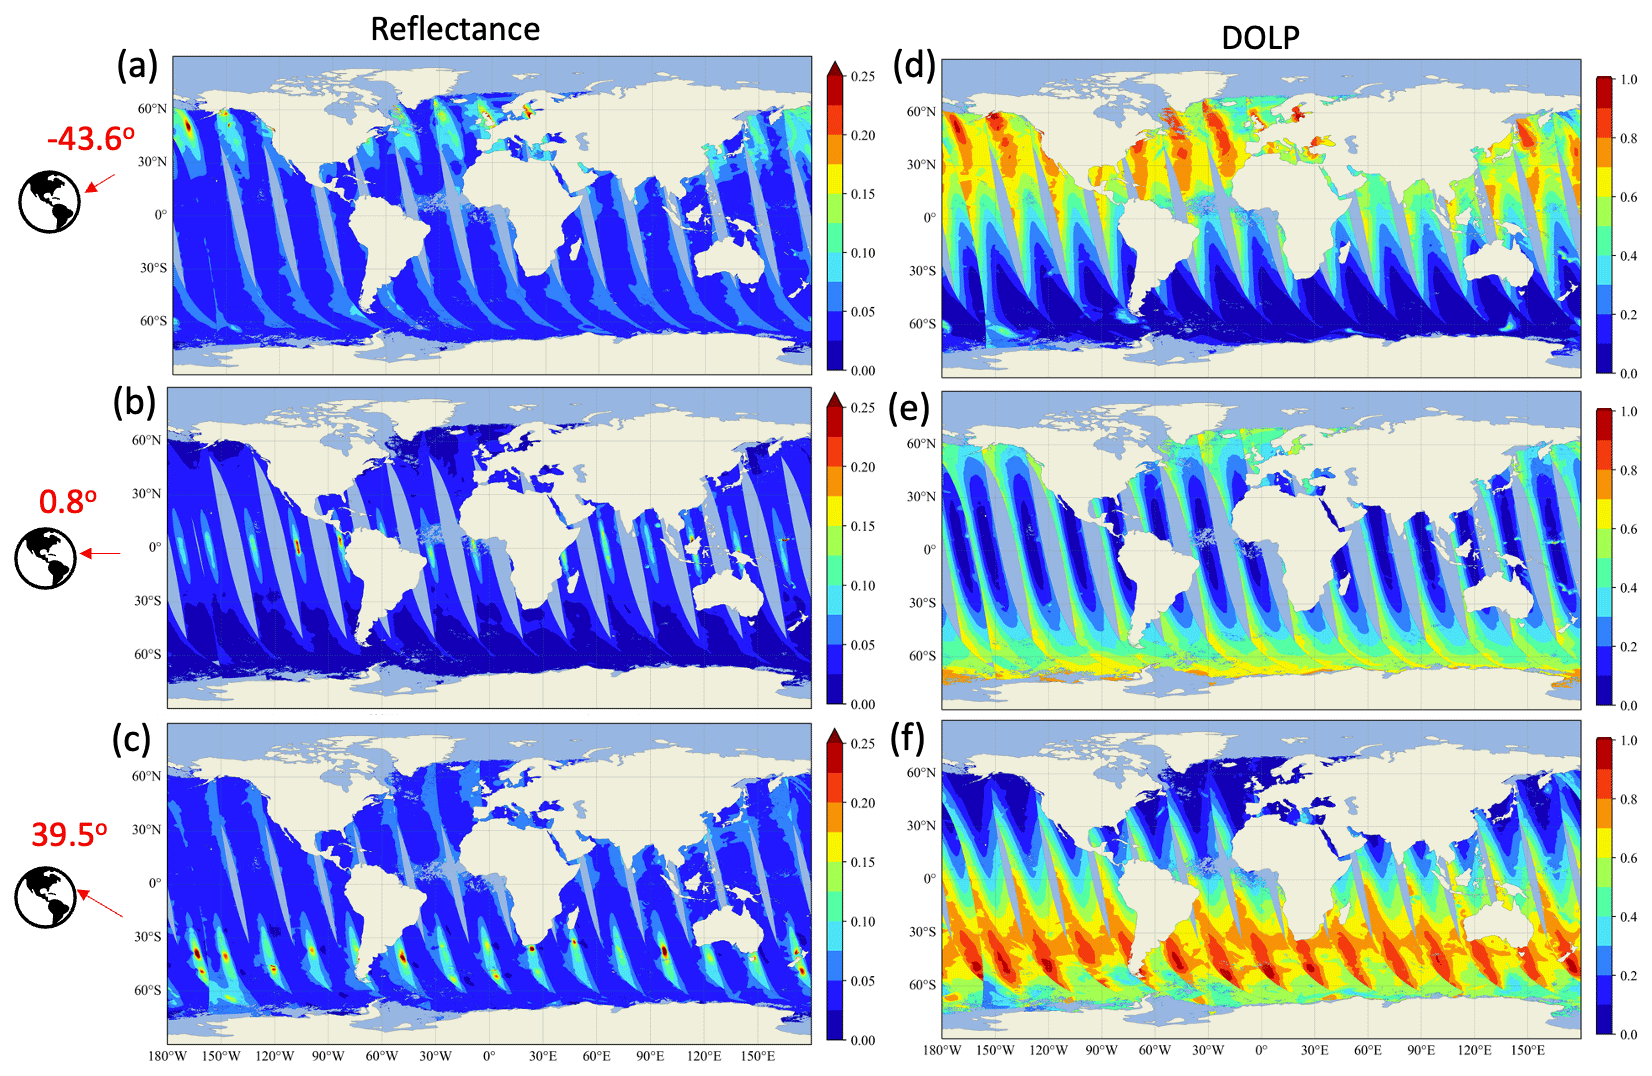
\includegraphics[width=0.8\linewidth,height=\textheight,keepaspectratio]{../chapters/../figure/validation_harp2_l1c.png}

}

\caption{\label{fig-validation_harp2_l1c}Global HARP2 simulation (550
nm): reflectance (a--c) and DoLP (d--f) from 15 orbits on 21 March 2022,
showing three along-track viewing angles. Figure is adopted from M. Gao
et al. (2023)}

\end{figure}%

\section{Geophysical retrievals with pixel-wise
uncertainty}\label{geophysical-retrievals-with-pixel-wise-uncertainty}

Based on the synthetic data, retrieval results as shown in
Figure~\ref{fig-validation_harp2_l2} demonstrate strong agreement with
truth and meaningful uncertainty estimates:

\begin{itemize}
\tightlist
\item
  AOD (550 nm) is retrieved with high accuracy and low spatial error.\\
\item
  Multiple geophysical variables are retrieved simultaneously, with ALH
  shown as an example.\\
\item
  Pixel-wise uncertainty reflects scene dependence, with larger values
  at low AOD and limited angular sampling.
\end{itemize}

\begin{figure}

\centering{

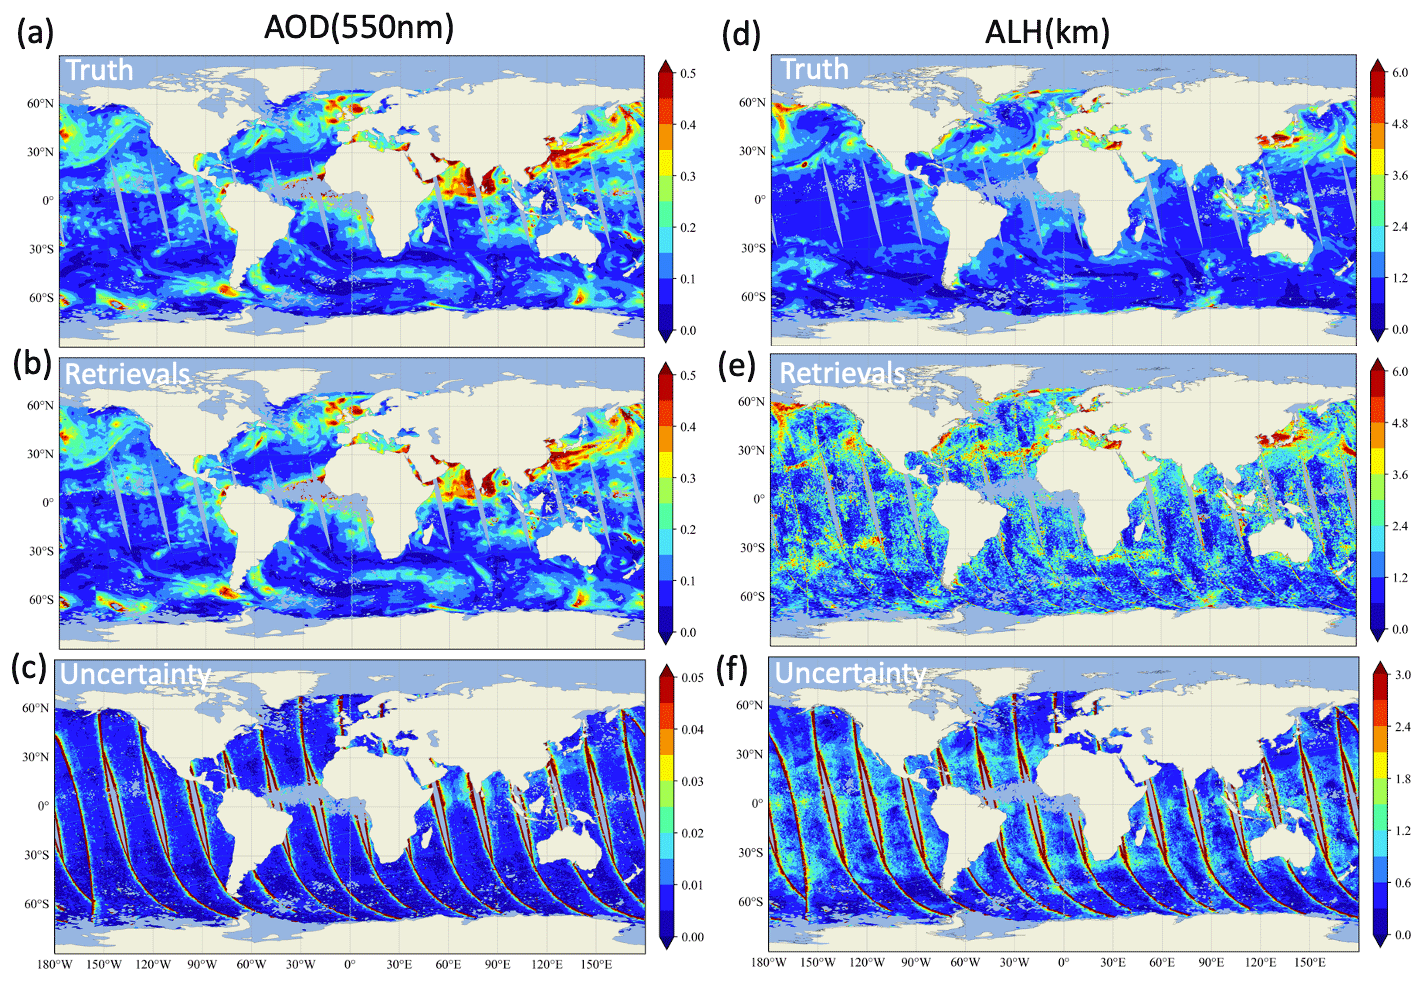
\includegraphics[width=0.8\linewidth,height=\textheight,keepaspectratio]{../chapters/../figure/validation_harp2_l2.png}

}

\caption{\label{fig-validation_harp2_l2}Retrieval performance: AOD (550
nm) and ALH showing retrieval, truth, and uncertainty (a--c, d--f).
Figure is adopted from M. Gao et al. (2023)}

\end{figure}%

\section{Uncertainty closure
analysis}\label{uncertainty-closure-analysis}

Theoretical uncertainties are derived from error propagation, while
realized uncertainties are computed from retrieval--truth differences.
Their comparisons are shown in Figure~\ref{fig-validation_harp2_unc},

\begin{itemize}
\tightlist
\item
  Good agreement for aerosol optical and microphysical properties,
  especially at moderate to high AOD.\\
\item
  Decreasing uncertainty with increasing aerosol loading.\\
\item
  Underestimation of uncertainty in low-AOD conditions and for weakly
  constrained parameters.
\end{itemize}

\begin{figure}

\centering{

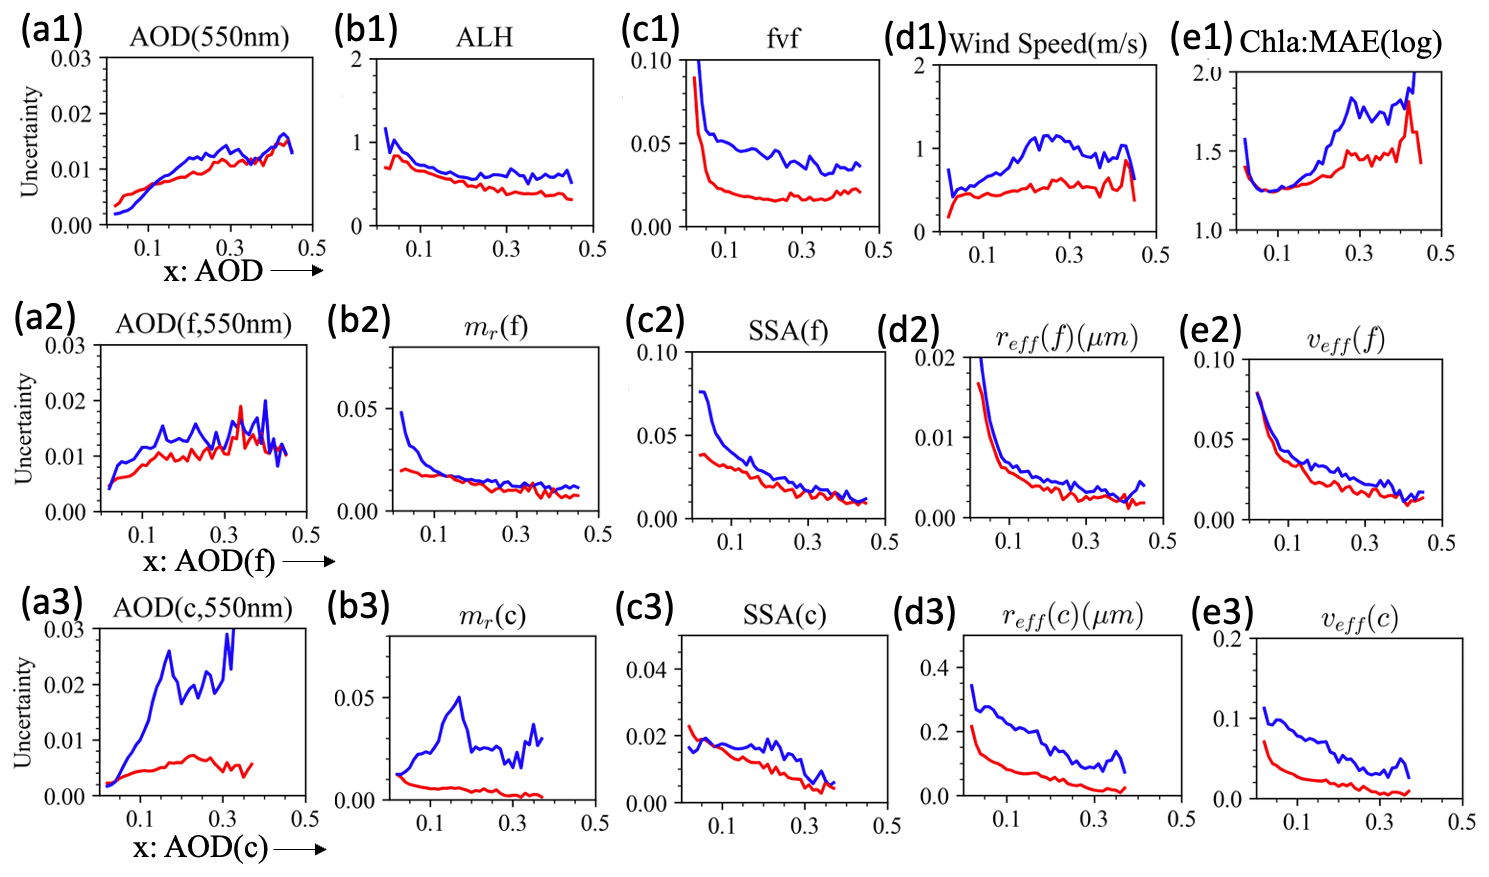
\includegraphics[width=0.9\linewidth,height=\textheight,keepaspectratio]{../chapters/../figure/validation_harp2_unc.png}

}

\caption{\label{fig-validation_harp2_unc}Theoretical (red) vs.~retrieved
(blue) uncertainties as a function of AOD for AOD, SSA, mr, reff, veff,
wind speed, and Chl a. AOD ranges from 0.01--0.45 (Δ=0.01). Figure is
adopted from M. Gao et al. (2023)}

\end{figure}%

\section{Summary}\label{summary}

\begin{itemize}
\tightlist
\item
  Synthetic data provide realistic multi-angle polarimetric
  observations.\\
\item
  L2 retrievals achieve high accuracy for key variables (especially
  AOD).\\
\item
  Pixel-level uncertainties are physically meaningful and scene
  dependent.\\
\item
  Uncertainty estimates are generally consistent with actual errors,
  with known limitations.
\end{itemize}

These results define a pre-launch benchmark for HARP2 L2 validation
using DITL data.

\bookmarksetup{startatroot}

\chapter{SPEXone aerosol and ocean product validation (V3.0 Provisional
data)}\label{spexone-aerosol-and-ocean-product-validation-v3.0-provisional-data}

This page summarizes validation results for aerosol and ocean products
retrieved from the PACE multi-angle polarimeters using the
\textbf{FastMAPOL} algorithm, with emphasis on \textbf{SPEXone} aerosol
optical properties and ocean remote-sensing reflectance (\(R_{rs}\)).

FastMAPOL performs coupled aerosol--surface retrievals using an
optimal-estimation framework accelerated by deep neural network forward
models. This page focuses only on the validation results and their
interpretation.

\textbf{More validation results are available in (\textbf{Gao:2026aa?}),
and will be available in PACE validation page. A similar study will be
conducted on HARP2}

\section{Summary Information}\label{summary-information-1}

\begin{itemize}
\tightlist
\item
  \textbf{FastMAPOL version:} v3.0\\
\item
  \textbf{Data period:} 2024/03--2025/12\\
\item
  \textbf{Reference:} AERONET v3, Level 1.5\\
\item
  \textbf{Page updated:} March 4, 2026
\end{itemize}

\section{Retrieval Products
Evaluated}\label{retrieval-products-evaluated}

\subsection{Aerosol}\label{aerosol}

\begin{itemize}
\tightlist
\item
  Total, fine-mode, and coarse-mode aerosol optical depth (AOD)
\item
  Total, fine-mode, and coarse-mode single-scattering albedo (SSA)
\end{itemize}

\subsection{Ocean}\label{ocean}

\begin{itemize}
\tightlist
\item
  Ocean remote-sensing reflectance (\(R_{rs}\))
\end{itemize}

\section{Validation Strategy}\label{validation-strategy}

Validation is organized into three levels:

\begin{enumerate}
\def\labelenumi{\arabic{enumi}.}
\item
  \textbf{Global Level-3 assessment}\\
  Evaluate large-scale spatial and seasonal patterns as shown below.
\item
  \textbf{Global aerosol validation}\\
  Compare retrievals with AERONET observations, please refer to
  (\textbf{Gao:2026aa?})
\item
  \textbf{Joint aerosol--ocean validation}\\
  Evaluate aerosol and \(R_{rs}\) simultaneously using AERONET-OC
  matchups, , please refer to (\textbf{Gao:2026aa?})
\end{enumerate}

The objective is to assess both the physical realism of the retrieved
fields and the consistency of aerosol and ocean products.

\section{Global Level-3 Products}\label{global-level-3-products}

\subsection{Aerosol Products (556 nm)}\label{aerosol-products-556-nm}

Global distributions of total, fine-mode, and coarse-mode AOD and SSA at
556 nm:

\begin{figure}[H]

{\centering \pandocbounded{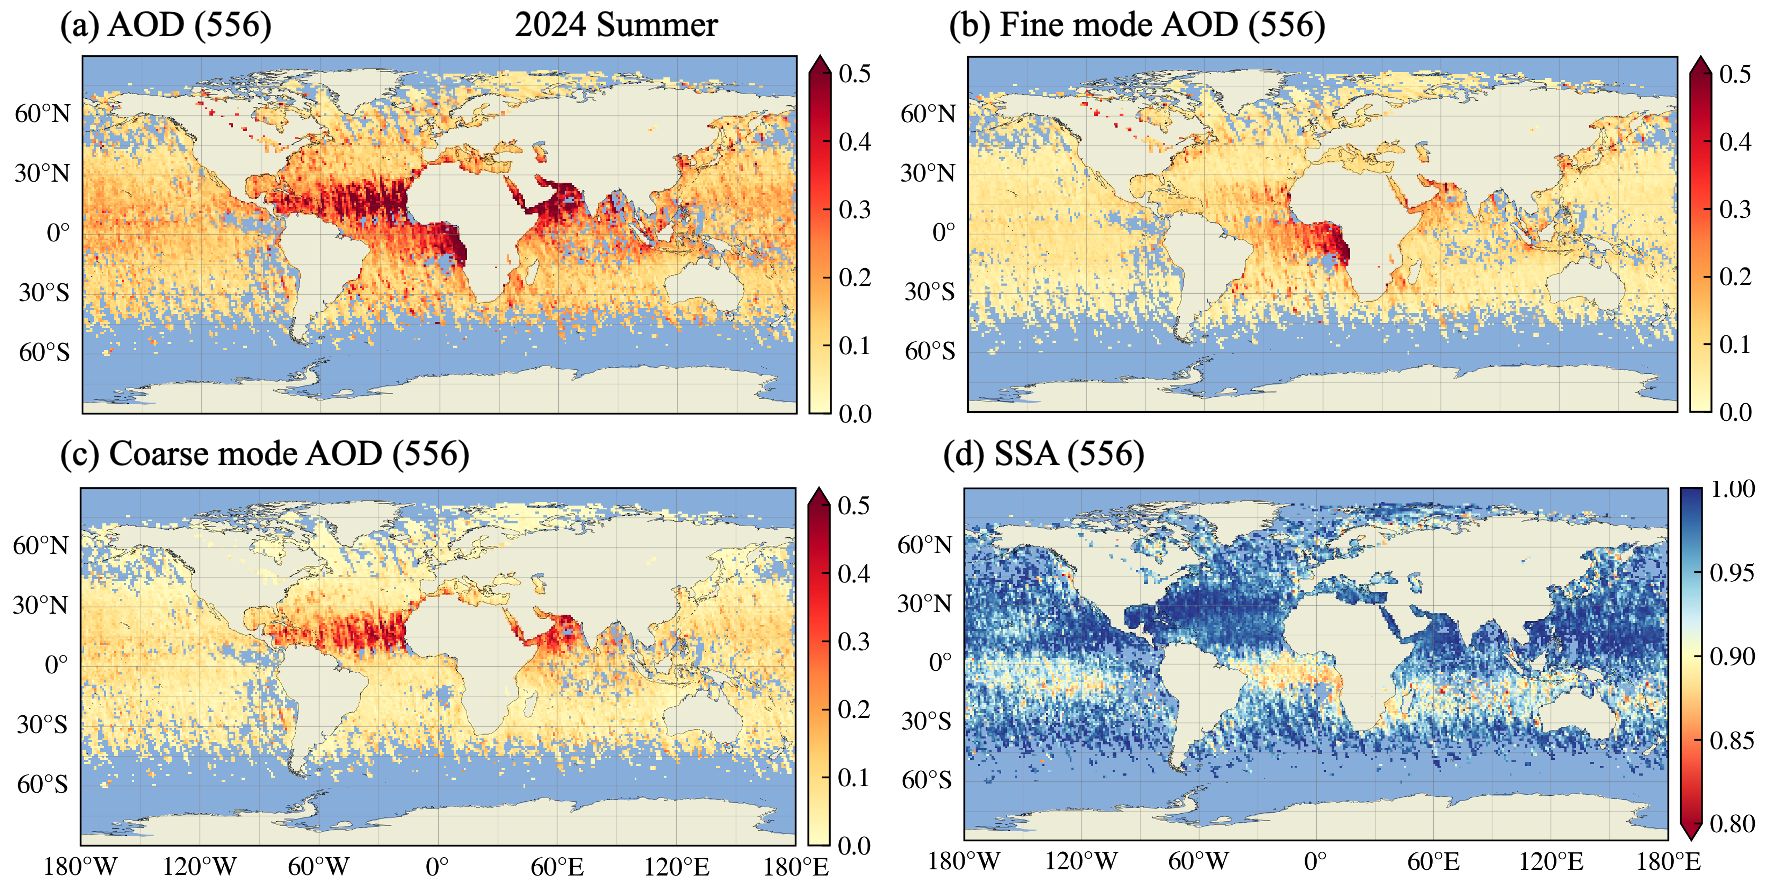
\includegraphics[keepaspectratio]{../chapters/../figure/validation_spexone_fig_15_0.04/fig_l3_aerosol_556.png}}

}

\caption{Global aerosol products}

\end{figure}%

\begin{center}\rule{0.5\linewidth}{0.5pt}\end{center}

\subsection{Ocean Products}\label{ocean-products}

Global distributions of \(R_{rs}\) (443, 556, 667 nm) and
chlorophyll-\emph{a}:

\begin{figure}[H]

{\centering \pandocbounded{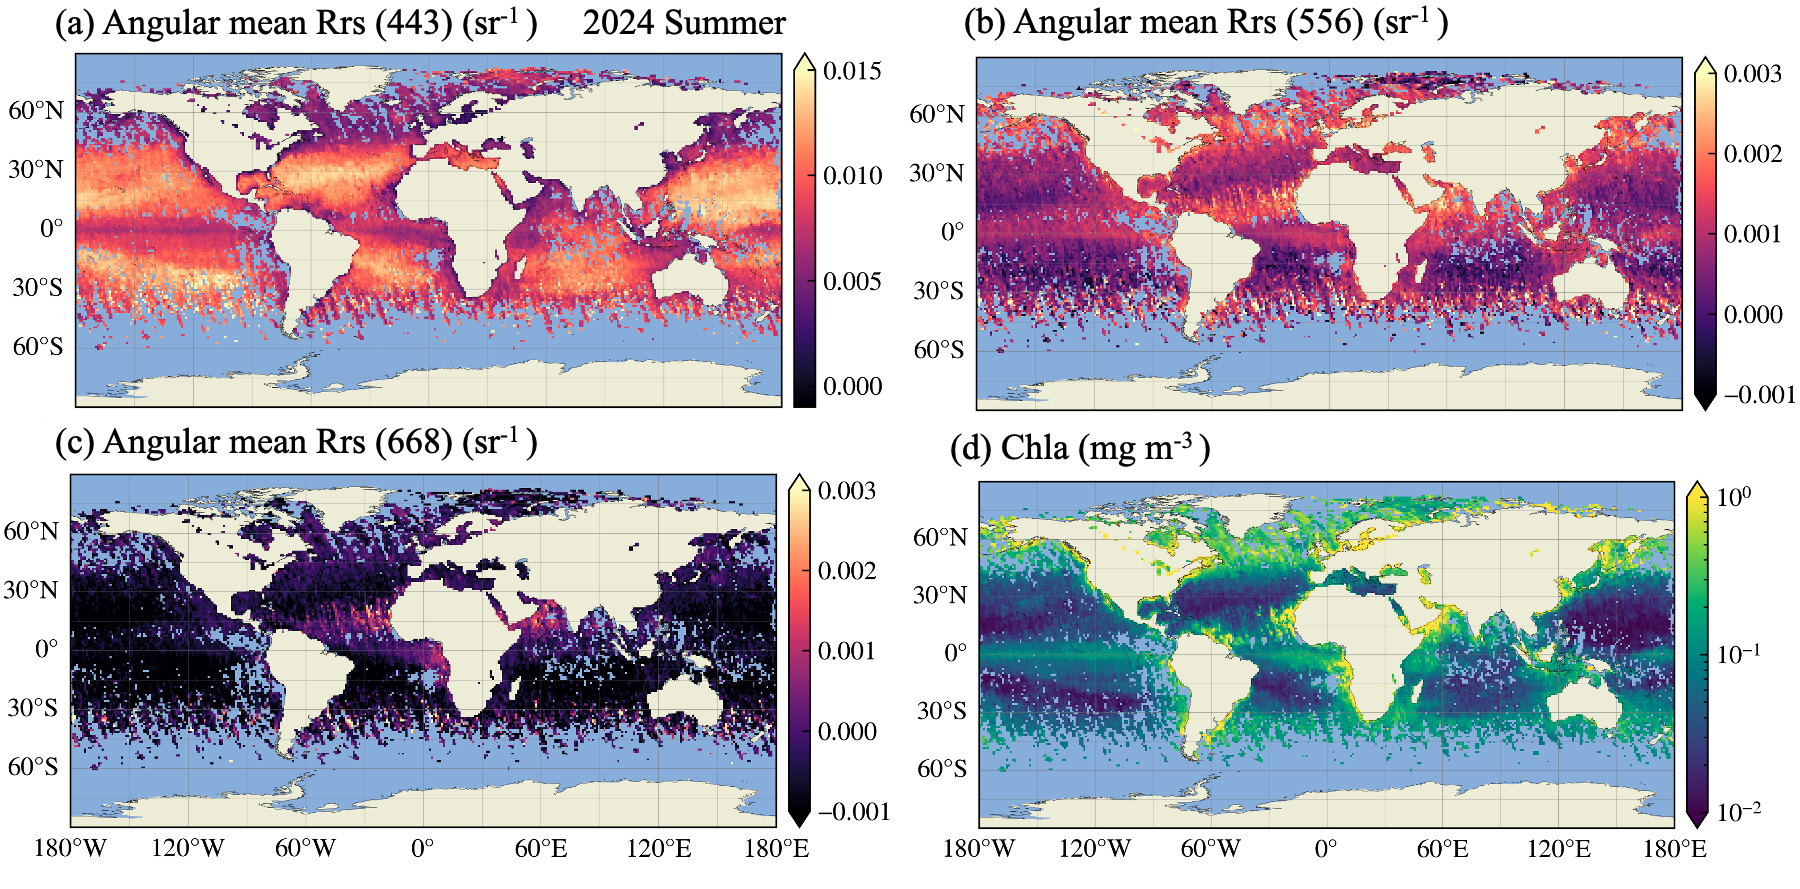
\includegraphics[keepaspectratio]{../chapters/../figure/validation_spexone_fig_15_0.04/fig_l3_rrs.png}}

}

\caption{Global ocean products}

\end{figure}%

The retrieved \(R_{rs}\) contains spectral and angular dimensions. The
results shown here represent the BRDF-corrected angular mean.

\textbf{Key result:}\\
The global distributions show realistic spatial and seasonal patterns,
indicating effective separation of atmospheric and oceanic retrieval
components.

\bookmarksetup{startatroot}

\chapter{Jupyter notebook tutorials}\label{jupyter-notebook-tutorials}

\section{L1}\label{l1}

\section{L2}\label{l2}

\section{L3}\label{l3}

\cleardoublepage
\phantomsection
\addcontentsline{toc}{part}{Appendices}
\appendix

\chapter{Technical Details}\label{technical-details}

This section provides detailed mathematical formulations, derivations,
and supporting information for the FastMAPOL algorithm. The material
presented here complements the main chapters and is intended for readers
who require a deeper understanding of the underlying theory,
assumptions, and implementation details.

The appendices include:

\begin{itemize}
\tightlist
\item
  Detailed formulations of aerosol size distributions and their
  moments\\
\item
  Derivations of lidar-related quantities, including lidar ratio and
  depolarization\\
\item
  Inversion methods connecting bulk aerosol properties to submode
  representations\\
\item
  Treatment of aerosol mixing and component partitioning\\
\item
  Pixel-level and correlated uncertainty analysis\\
\item
  Surface reflectance models for ocean and land
\end{itemize}

These technical details are not required for general use or
interpretation of the FastMAPOL products but are essential for algorithm
development, validation, and advanced scientific analysis.

All equations and formulations follow the conventions introduced in the
main text unless otherwise noted.

\chapter{Aerosol characterization : size distribution and
representation}\label{aerosol-characterization-size-distribution-and-representation}

FastMAPOL supports several aerosol representations with increasing
complexity:

\begin{itemize}
\tightlist
\item
  \textbf{Aer-1:} five predefined log-normal modes
\item
  \textbf{Aer-2:} six predefined log-normal modes
\item
  \textbf{Aer-3:} aerosol components represented by chemical composition
\end{itemize}

These aerosol models share a common mathematical framework for size
integration, mode summation, optical properties, and bulk aerosol
products. This chapter summarizes the formulation used to connect the
retrieved state variables to physically meaningful aerosol quantities,
including optical depth, effective radius, effective variance, fine-mode
fraction, and volume fraction. In this chapter, we focused on the first
two models.

\section{Overview}\label{overview-2}

The aerosol model formulation includes the following key elements:

\begin{itemize}
\tightlist
\item
  size integration over each particle size distribution
\item
  calculation of effective radius and effective variance
\item
  multi-mode considerations
\item
  derivation of aerosol products such as fine-volume fraction (FVF) and
  fine-mode fraction (FMF)
\end{itemize}

\section{Aerosol density
distributions}\label{aerosol-density-distributions}

\subsection{Conversion between volume and number density log-normal
distributions}\label{conversion-between-volume-and-number-density-log-normal-distributions}

Both the number density and the volume density can be represented by
log-normal distributions. The two forms are equivalent and can be
converted into each other by changing the mean radius and the
normalization constant.

For a monomodal system, the volume and number size distributions are
written as

\[
\frac{d V(r)}{d \ln r}= \frac{V_{0}}{\sqrt{2 \pi} \sigma_{v}} \exp\left[-\frac{(\ln r-\ln r_{v})^2}{2 \sigma_{v}^2}\right],
\]

\[
\frac{d N(r)}{d \ln r}= \frac{N_{0}}{\sqrt{2 \pi} \sigma_{n}} \exp\left[-\frac{(\ln r-\ln r_{n})^2}{2 \sigma_{n}^2}\right].
\]

Here, \(r_v\) and \(r_n\) are the mean radii for the volume and number
distributions, respectively, and \(\sigma_v\) and \(\sigma_n\) are the
corresponding logarithmic standard deviations. The formulation follows
Xu (2016, Appendix A6), with the corrected definition of \(\sigma\) as
confirmed by Pengwang Zhai through personal communication with Feng Xu.

Since particle volume and number are related by

\[
V=\frac{4\pi}{3}Nr^3,
\]

the corresponding differential distributions satisfy

\[
\frac{d V(r)}{d \ln r}=\frac{4\pi}{3} r^3 \frac{d N(r)}{d \ln r}.
\]

Using this relation, the following identities are obtained:

\[
\sigma_{n}=\sigma_{v}=\sigma,
\]

\[
r_{n}=r_{v} \exp(-3 \sigma^2),
\]

\[
N_{0}=V_{0} \frac{3}{4 \pi r_{v}^3}\exp(4.5 \sigma^2),
\]

\[
N_{0}=V_{0} \frac{3}{4 \pi r_{n}^3}\exp(-4.5 \sigma^2).
\]

These results are consistent with the derivation given by R.G. Grainger.
The last two expressions provide an internal consistency check.

\section{Optical depth}\label{optical-depth}

Using the conversion above, the column-integrated number density can be
expressed in terms of the column-integrated volume density as

\[
N_{0}=V_{0} \frac{3}{4 \pi r_{v}^3}\exp(4.5 \sigma^2).
\]

The aerosol optical depth is defined as

\[
\tau_a=\sum_{i=1}^{N_c} C_{ext,i} N_i,
\]

where \(C_{ext,i}\) is the extinction cross section of component \(i\)
in units of \(\mu m^2\), and \(N_i\) is the corresponding column number
density in units of \(\mu m^{-2}\).

Here, column number density is equivalent to vertically integrated
number density. If the local number density is \(n\) in units of
\(\mu m^{-3}\) and the layer thickness is \(z\) in units of \(\mu m\),
then

\[
N = n z.
\]

Using column volume density, the optical depth can be rewritten as

\[
\tau_a = \sum_{i=1}^{N_c} C_{ext,i} N_i,
\]

\[
\tau_a = \sum_{i=1}^{N_c} C_{ext,i} V_i \frac{3}{4 \pi r_{v}^3}\exp(4.5 \sigma^2),
\]

\[
\tau_a = \sum_{i=1}^{N_c} \left[C_{ext,i} \frac{3}{4 \pi r_{v}^3}\exp(4.5 \sigma^2)\right] V_i.
\]

The unit of column volume density is \(\mu m^3 \mu m^{-2}\), which
reduces to \(\mu m\).

If a maximum optical depth \(\tau_{max}\) is prescribed, then the
corresponding maximum allowed volume density for each component is

\[
V_i=\tau_{max}\left[C_{ext,i} \frac{3}{4 \pi r_{v}^3}\exp(4.5 \sigma^2)\right]^{-1},
\]

or equivalently

\[
V_i=\tau_{max} \exp(4.5 \sigma^2) \frac{4 \pi r_{v}^3}{3 C_{ext,i}}.
\]

A practical bound on \(V_i\) can be estimated at a reference wavelength
such as \(550 \, nm\) by computing extinction cross sections over the
expected refractive-index range for each mode. For the lower bound, one
may use a real refractive index close to that of water at \(550 \, nm\),
approximately 1.3.

In general, increasing the imaginary part of the refractive index
increases the extinction cross section. For coarse particles, however,
the extinction is often much less sensitive to refractive index than to
particle size.

\section{Convention for size
distributions}\label{convention-for-size-distributions}

The size distributions may be defined with respect to either \(r\) or
\(\ln r\). These forms are related by

\[
\frac{d N(r)}{d r}=\frac{1}{r}\frac{d N(r)}{d \ln r},
\]

\[
\frac{d V(r)}{d r}=\frac{1}{r}\frac{d V(r)}{d \ln r}.
\]

This distinction is important when comparing formulations from different
references or numerical implementations.

\section{Moments of the particle size
distribution}\label{moments-of-the-particle-size-distribution}

For later use, define the \(k\)th moment of the number size distribution
as

\[
m_k=\int_{0}^{\infty} r^k \frac{d N(r)}{d r} \, d r,
\]

which is equivalently

\[
m_k=\int_{-\infty}^{\infty} r^k \frac{d N(r)}{d \ln r} \, d \ln r.
\]

For a log-normal number distribution,

\[
m_k=N_0 r_n^k \exp\left(\frac{k^2}{2} \sigma^2\right).
\]

The dimension is consistent: \(m_k\) has units of \(r^k\), while
\(\sigma\) is dimensionless.

Substituting the number-volume conversion into the moment expression
gives

\[
m_k=N_0 r_n^k \exp\left(\frac{k^2}{2} \sigma^2\right),
\]

\[
m_k=V_{0} \frac{3}{4 \pi r_{v}^3}\exp(4.5 \sigma^2)r^k_{v} \exp(-3k \sigma^2) \exp\left(\frac{k^2}{2} \sigma^2\right),
\]

and therefore

\[
m_k=V_{0} \frac{3}{4 \pi} r^{k-3}_v\exp\left[\frac{(k-3)^2\sigma^2}{2} \right].
\]

This result preserves dimensional consistency because \(V_0\) carries
the dimension of \(r^3\).

A useful special case is \(k=3\), for which

\[
m_3=\frac{3V_0}{4\pi}.
\]

Thus, the third moment depends directly on the total particle volume.

\section{\texorpdfstring{Effective radius and effective variance in
terms of
\(dN/d\ln r\)}{Effective radius and effective variance in terms of dN/d\textbackslash ln r}}\label{effective-radius-and-effective-variance-in-terms-of-dndln-r}

The effective radius, or area-weighted mean radius, is defined as

\[
r_{eff}=\frac{\int_{r_1}^{r_2} r \, r^2 (dN(r)/dr) \, dr}{\int_{r_1}^{r_2} r^2 (dN(r)/dr) \, dr}
=\frac{m_3}{m_2}.
\]

The weighting by particle area reflects the fact that radiative
extinction is approximately proportional to particle cross-sectional
area.

The effective variance is defined as

\[
\nu_{eff}=\frac{\int_{r_1}^{r_2}(r-r_{eff})^2 r^2 (dN(r)/dr) \, dr}
{r^2_{eff} \int_{r_1}^{r_2}r^2 (dN(r)/dr) \, dr},
\]

which can be written in terms of moments as

\[
\nu_{eff}= \frac{m_4 m_2}{m_3^2}-1.
\]

This expression is equally valid for distributions written in terms of
\(dN(r)/d\ln r\).

For a log-normal number distribution

\[
\frac{d N(r)}{d \ln r}=\frac{N_0}{\sqrt{2 \pi} \sigma} \exp\left[-\frac{(\ln r-\ln r_n)^2}{2 \sigma^2}\right],
\]

the effective radius and effective variance are

\[
r_{eff}=r_n \exp\left(\frac{5}{2} \sigma^2\right),
\]

\[
\nu_{eff}=\exp (\sigma^2)-1.
\]

Using the relation between number-mean and volume-mean radius,

\[
r_{eff}=r_n \exp(2.5 \sigma^2),
\]

\[
r_{eff}=r_v \exp(-3 \sigma^2) \exp(2.5 \sigma^2),
\]

\[
r_{eff}=r_v \exp(-0.5 \sigma^2).
\]

Thus, the effective radius is always larger than the number-mean radius
and smaller than the volume-mean radius.

For small \(\sigma^2\), the approximations

\[
\nu_{eff}=\exp (\sigma^2)-1 \approx \sigma^2
\]

and

\[
r_{eff}= r_v \exp(-0.5 \sigma^2) \approx r_v
\]

show that the effective variance is approximately the square of the
logarithmic standard deviation, while the effective radius approaches
the volume-mean radius.

\section{\texorpdfstring{Effective radius and variance in terms of
\(dV/d\ln r\)}{Effective radius and variance in terms of dV/d\textbackslash ln r}}\label{effective-radius-and-variance-in-terms-of-dvdln-r}

Because the retrieval state is often expressed in terms of volume
density, it is useful to write effective radius and effective variance
directly in terms of the volume distribution.

Starting from

\[
\frac{d V(r)}{d \ln r}=\frac{4\pi}{3} r^3 \frac{d N(r)}{d \ln r},
\]

the effective radius becomes

\[
r_{eff}=\frac{\int_{\ln r_1}^{\ln r_2} (dV(r)/d\ln r) \, d\ln r}
{\int_{\ln r_1}^{\ln r_2} r^{-1} (dV(r)/d\ln r) \, d\ln r}.
\]

Define the moments of the volume distribution as

\[
m'_k = \int_{\ln r_1}^{\ln r_2} r^k \left(\frac{dV(r)}{d\ln r}\right) d\ln r.
\]

Then

\[
r_{eff}= \frac{m'_0}{m'_{-1}}.
\]

Similarly, the effective variance becomes

\[
\nu_{eff}=\frac{\int_{\ln r_1}^{\ln r_2}(r-r_{eff})^2 r^{-1} (dV(r)/d\ln r) \, d\ln r}
{r^2_{eff} \int_{\ln r_1}^{\ln r_2} r^{-1} (dV(r)/d\ln r) \, d\ln r},
\]

which simplifies to

\[
\nu_{eff}= \frac{m'_{-1} m'_1}{m'^2_0}-1.
\]

For discrete numerical implementation, the moment may be written
schematically as

\[
m'_k \approx \sum_i r(i)^k v(i,j),
\]

where \(i\) indexes the size grid and \(j\) indexes pixel or retrieval
location. The constant increment \(d\ln r\) is omitted here for brevity.

For a log-normal volume distribution,

\[
m'_k =V_{0} \frac{3}{4 \pi} r^{k}_v\exp\left[\frac{k^2\sigma^2}{2} \right].
\]

For a multimode distribution, the effective quantities become

\[
r_{eff}=\frac{\sum_i m_{3,i}}{\sum_i m_{2,i}}
\]

and

\[
\nu_{eff}=\frac{\sum_i m_{4,i} \sum_i m_{2,i}}{(\sum_i m_{3,i})^2}-1
\]

when expressed through number-density moments, or equivalently

\[
r_{eff}=\frac{\sum_i m'_{0,i}}{\sum_i m'_{-1,i}},
\]

\[
\nu_{eff}=\frac{\sum_i m'_{1,i} \sum_i m'_{-1,i}}{(\sum_i m'_{0,i})^2}-1
\]

when expressed through volume-density moments.

\section{Multi-mode distributions}\label{multi-mode-distributions}

When the aerosol is represented as a sum of log-normal modes,

\[
\frac{d V(r)}{d \ln r}= \sum_i \frac{V_{0,i}}{\sqrt{2 \pi} \sigma_{v,i}} \exp\left[-\frac{(\ln r-\ln r_{v,i})^2}{2 \sigma_{v,i}^2}\right],
\]

\[
\frac{d N(r)}{d \ln r}= \sum_i \frac{N_{0,i}}{\sqrt{2 \pi} \sigma_{n,i}} \exp\left[-\frac{(\ln r-\ln r_{n,i})^2}{2 \sigma_{n,i}^2}\right].
\]

For each mode, the conversion relations are

\[
\sigma_{n,i}=\sigma_{v,i}=\sigma_i,
\]

\[
r_{n,i}=r_{v,i} \exp(-3 \sigma_{i}^2),
\]

\[
N_{0,i}=V_{0,i} \frac{3}{4 \pi r_{v,i}^3}\exp(4.5 \sigma_{i}^2),
\]

\[
N_{0,i}=V_{0,i} \frac{3}{4 \pi r_{n,i}^3}\exp(-4.5 \sigma_{i}^2).
\]

The distinction between number weighting and volume weighting remains
important, since the same physical aerosol can have different mean radii
depending on which representation is used.

For the volume-mode parameterization adopted from Dubovik et al. (2011)
and Xu et al. (2016), the nominal mode radii are

\[
0.1,\ 0.1732,\ 0.3,\ 1.0,\ 2.9 \ \mu m
\]

with logarithmic standard deviations

\[
0.35,\ 0.35,\ 0.35,\ 0.5,\ 0.5.
\]

The impact of the number of modes are further discussed by Fu:2020aa. We
adopted this approach as default aerosol model (Aer-1). Meng Gao et al.
(2018) add an additional coarse mode to deal with the larger aerosol
size when using the SWIR bands from RSP. The nomial radii and standard
deviations are 8.4 \(\mu m\) and 0.5, which is called (Aer-2).

\section{Averaged extinction cross
section}\label{averaged-extinction-cross-section}

When extinction is averaged over a volume-based aerosol model, number
density must first be recovered from the volume density.

For the same total particle volume, a fine mode contains far more
particles than a coarse mode. As a result, fine-mode particles can
dominate number-weighted optical properties even when their volume
contribution is modest.

For two modes, the total extinction can be written as

\[
C_{ext,t}=C_{ext,f} n_f+C_{ext,c} n_c,
\]

or in terms of volume density,

\[
C_{ext,t}= C_{ext,f} \frac{3 V_f}{4\pi r^3_{v,f}}\exp(4.5 \sigma^2_f)+
C_{ext,c} \frac{3 V_c}{4\pi r^3_{v,c}}\exp(4.5 \sigma^2_c).
\]

To compare fine- and coarse-mode contributions, consider the ratio

\[
\frac{C_{ext,f} \frac{3 V_f}{4\pi r^3_{v,f}}\exp(4.5 \sigma^2_f)}
{C_{ext,c} \frac{3 V_c}{4\pi r^3_{v,c}}\exp(4.5 \sigma^2_c)}.
\]

If the logarithmic standard deviations are assumed equal, this ratio
simplifies to an expression proportional to

\[
\frac{V_f}{V_c}\frac{Q_{ext,f} r_{v,c}}{Q_{ext,c} r_{v,f}},
\]

showing explicitly how fine-mode dominance arises from both larger
number concentration per unit volume and the size dependence of
extinction efficiency.

\section{Effective radius and variance for multimode
aerosols}\label{effective-radius-and-variance-for-multimode-aerosols}

The total number density and total volume density are

\[
N_0=\sum_i N_{0,i},
\]

\[
V_0=\sum_i V_{0,i}.
\]

The effective radius and effective variance of the combined distribution
are

\[
r_{eff}=\frac{\sum_i m_{3,i}}{\sum_i m_{2,i}},
\]

\[
\nu_{eff}=\frac{\sum_i m_{4,i} \sum_i m_{2,i}}{(\sum_i m_{3,i})^2}-1.
\]

\subsection{Sensitivity to component
volume}\label{sensitivity-to-component-volume}

To propagate retrieval uncertainty from mode volumes to bulk effective
properties, derivatives with respect to \(V_j\) are required.

For effective radius,

\[
\frac{\partial r_{eff}}{\partial V_{j}} =
\frac{1}{\sum_i  m_{2,i}}\frac{\partial m_{3,j}}{\partial V_j}- 
\frac{\sum_i m_{3,i}}{(\sum_i m_{2,i})^2}\frac{\partial m_{2,j}}{\partial V_j},
\]

which can be written as

\[
\frac{\partial r_{eff}}{\partial V_{j}} =
r_{eff} \left(\frac{m'_{3,j}}{\sum_i  m_{3,i}}-\frac{m'_{2,j}}{\sum_i  m_{2,i}}\right).
\]

For effective variance,

\[
\frac{\partial \nu_{eff}}{\partial V_j}=
\frac{\sum_i m_{2,i}}{(\sum_i m_{3,i})^2}\frac{\partial m_{4,j}}{\partial V_j}+
\frac{\sum_i m_{4,i}}{(\sum_i m_{3,i})^2}\frac{\partial m_{2,j}}{\partial V_j}
-2\frac{\sum_i m_{4,i} \sum_i m_{2,i}}{(\sum_i m_{3,i})^3}\frac{\partial m_{3,j}}{\partial V_j},
\]

or equivalently

\[
\frac{\partial \nu_{eff}}{\partial V_j}=
(\nu_{eff}+1) \left(\frac{m'_{4,j}}{\sum_i  m_{4,i}}+\frac{m'_{2,j}}{\sum_i m_{2,i}} 
-2\frac{m'_{3,j}}{\sum_i  m_{3,i}}\right).
\]

Here the derivative of the moment with respect to component volume is

\[
m'_{k,j}=\frac{\partial m_{k,j}}{\partial V_j}=\frac{m_{k,j}}{V_j},
\]

which gives

\[
m'_{k,j}=\frac{3}{4 \pi}
r^{k-3}_{v,j} \exp\left[\frac{(k-3)^2}{2} \sigma_j^2\right].
\]

For \(k=3\), this derivative is constant because \(m_3\) depends
linearly on volume and not on radius.

\section{Physical interpretation of low-order
moments}\label{physical-interpretation-of-low-order-moments}

For a volume-based log-normal mode, the low-order moments are

\[
m_{2,i}=\frac{3}{4\pi} V_i r_{v,i}^{-1} \exp(\sigma_i^2/2),
\]

\[
m_{3,i}=\frac{3}{4\pi} V_i,
\]

\[
m_{4,i}=\frac{3}{4\pi} V_i r_{v,i} \exp(\sigma_i^2/2).
\]

For a single mode, these lead directly to

\[
r_{eff}=\frac{m_3}{m_2}=r_v \exp(-\sigma^2/2),
\]

\[
\nu_{eff}=\frac{m_4 m_2}{m_3^2}-1=\exp (\sigma^2)-1.
\]

For a multimode aerosol,

\[
\sum_i m_{3,i}=\frac{3}{4\pi}\sum_i V_i=\frac{3}{4\pi} V_0,
\]

so the summed third moment is proportional to the total particle volume.

Within a fine-mode or coarse-mode subset, \(m_2\) emphasizes smaller
particles, whereas \(m_4\) emphasizes larger particles. This makes
effective radius and effective variance sensitive to the relative
partitioning among submodes, even when the logarithmic standard
deviation is fixed within that subset.

\section{Fine and coarse mode
partitions}\label{fine-and-coarse-mode-partitions}

To discuss fine-mode and coarse-mode aerosol separately, the mode
summation may be restricted to selected ranges.

For the Aer-1 and Aer-2 parameterization adopted here:

\begin{itemize}
\tightlist
\item
  \textbf{fine mode:} modes 1 to 3, with volume-mean radii from \(0.1\)
  to \(0.3 \, \mu m\)
\item
  \textbf{coarse mode:} modes 4 and above, with volume-mean radii from
  \(1.0\), \(2.9, (and 8.4) \mu m\)
\end{itemize}

Although the first three fine modes share the same logarithmic standard
deviation, their effective variance can still change because the bulk
quantity depends on the relative partitioning among the mode volumes.

\section{Phase-matrix averaging}\label{phase-matrix-averaging}

The total number density may be represented as a weighted sum of
component size distributions,

\[
n(r)=\sum_i c_i n_i(r),
\]

with

\[
\sum_i c_i =1.
\]

The corresponding size-averaged phase matrix is then

\[
P(\Omega)_{avg}=\int d r \, n(r) P(\Omega;r),
\]

which can be expanded as

\[
P(\Omega)_{avg}= \sum_i c_i \int d r \, n_i(r) P(\Omega;r)
\]

and written as

\[
P(\Omega)_{avg}= \sum_i c_i P_i (\Omega).
\]

If \(P_i\) denotes the size-averaged phase matrix of component \(i\),
then the total phase matrix is a weighted sum over components. If
normalized phase matrices \(\tilde{P}_i\) are used, then the weighting
must be consistent with the corresponding scattering cross sections.

In practice, this requires confirming the normalization convention of
the scattering subroutine, such as \texttt{spher\_interface}.

\section{Additional notes on units}\label{additional-notes-on-units}

The column number density may also be written as

\[
N_0=n_0 \delta l,
\]

where \(\delta l\) is the aerosol layer thickness.

In log-normal expressions, the absolute unit of radius does not matter
as long as \(r\) and the mean radius use the same unit, since

\[
\ln r-\ln r_m=\ln(r/r_m).
\]

Both the logarithmic variance and the effective variance are
dimensionless.

\section{Optical depth at different
wavelengths}\label{optical-depth-at-different-wavelengths}

If the aerosol loading is parameterized at a reference wavelength, such
as \(555 \, nm\), then the corresponding number density can be defined
as

\[
n_i=\frac{\tau_{555nm}}{C_{ext,555nm}}.
\]

The optical depth at any other wavelength is then

\[
\tau_{\lambda}=n_i C_{ext,\lambda}.
\]

This relation is useful when the state variable is defined through
reference-wavelength optical depth while the forward model requires
spectrally varying extinction.

\section{Aerosol products}\label{aerosol-products}

The aerosol model supports the derivation of bulk products from the
retrieved mode volumes and optical properties. These include, for
example:

\begin{itemize}
\tightlist
\item
  \textbf{FMF:} fine-mode fraction, typically defined from fine-mode
  optical depth relative to total optical depth at a reference
  wavelength
\item
  \textbf{FVF:} fine-volume fraction, defined from fine-mode particle
  volume relative to total particle volume
\item
  effective radius and effective variance for fine, coarse, or total
  aerosol
\item
  spectrally resolved optical depth and related intensive properties
\end{itemize}

The exact definition of each product depends on the chosen aerosol
representation and on whether the partitioning is performed by mode, by
size, or by composition.

\section{Summary}\label{summary-1}

The aerosol model is built on a consistent log-normal framework that
links retrieved mode volumes to number density, optical depth, size
moments, and bulk aerosol properties. The volume-based representation is
particularly convenient for retrieval, while the number-based
representation remains useful for interpreting extinction and other
radiatively weighted quantities. The relationships summarized here
provide the basis for size integration, mode summation, and the
calculation of operational aerosol products in FastMAPOL.

\chapter{Aerosol characterization: Lidar ratio and
depolarization}\label{aerosol-characterization-lidar-ratio-and-depolarization}

\section{Overview}\label{overview-3}

The aerosol retrieval framework provides extinction and scattering
properties together with the angular scattering phase matrix. These
quantities can be used to derive lidar observables, in particular the
\textbf{lidar ratio} and the \textbf{linear depolarization ratio}.

This chapter summarizes the mathematical connection between the
retrieved aerosol optical properties and the lidar-relevant quantities.
The focus here is on the forward relationships from extinction and phase
matrix elements to the lidar ratio and depolarization, for total aerosol
as well as for fine and coarse aerosol partitions.

\section{Scattering and extinction
quantities}\label{scattering-and-extinction-quantities}

For a given aerosol population, let

\[
C_{ext}
\]

denote the extinction coefficient or extinction cross section, and let

\[
C_{sca}
\]

denote the scattering coefficient or scattering cross section.

The single-scattering albedo is defined as

\[
\omega_0 = \frac{C_{sca}}{C_{ext}}.
\]

For a partitioned aerosol model, the same definition applies separately
to the fine mode, coarse mode, and total aerosol:

\[
\omega_{0,f} = \frac{C_{sca,f}}{C_{ext,f}},
\]

\[
\omega_{0,c} = \frac{C_{sca,c}}{C_{ext,c}},
\]

\[
\omega_{0} = \frac{C_{sca}}{C_{ext}}.
\]

Although the single-scattering albedo is not itself a lidar product, it
provides useful context because the backscatter signal depends on the
angular redistribution of the scattered power, while extinction controls
the attenuation of the lidar beam.

\section{Phase matrix and backscattering
geometry}\label{phase-matrix-and-backscattering-geometry}

The scattering properties of the aerosol are described by the phase
matrix, written here as

\[
\mathbf{P}(\Theta),
\]

where \(\Theta\) is the scattering angle. In the standard convention for
randomly oriented particles with mirror symmetry, the phase matrix
contains elements such as

\[
P_{11}(\Theta), \qquad P_{22}(\Theta),
\]

together with the other Mueller-matrix elements.

For lidar applications, the relevant direction is the \textbf{exact
backscattering direction}, corresponding to

\[
\Theta = 180^\circ.
\]

In the numerical implementation, this corresponds to the last angular
index of the phase-matrix array. Therefore, the backscatter-related
quantities are obtained from the phase matrix evaluated at
\(\Theta = 180^\circ\).

Let

\[
P_{11}(180^\circ)
\]

and

\[
P_{22}(180^\circ)
\]

denote the first and second diagonal phase-matrix elements at exact
backscatter.

\section{Relation between phase matrix and volume
backscatter}\label{relation-between-phase-matrix-and-volume-backscatter}

The lidar backscatter coefficient is proportional to the phase function
evaluated at the backscattering direction.

If the phase matrix is normalized such that

\[
\int_{4\pi} P_{11}(\Theta,\phi)\, d\Omega = 4\pi,
\]

then the backscatter coefficient is

\[
\beta = \frac{C_{sca}}{4\pi} P_{11}(180^\circ).
\]

Equivalently, if the retrieved quantity is an extinction coefficient
rather than a cross section, the same relation holds with coefficient
units instead of per-particle units. The key point is that the lidar
backscatter coefficient is proportional to the product of scattering
strength and the phase-matrix element in the exact backscattering
direction.

Thus, for fine mode, coarse mode, and total aerosol, one may write

\[
\beta_f = \frac{C_{sca,f}}{4\pi} P_{11,f}(180^\circ),
\]

\[
\beta_c = \frac{C_{sca,c}}{4\pi} P_{11,c}(180^\circ),
\]

\[
\beta = \frac{C_{sca}}{4\pi} P_{11}(180^\circ).
\]

If the retrieval outputs a matrix-valued quantity already scaled by
scattering coefficient, then the same formulas apply after confirming
the normalization convention of the stored matrix.

\section{Lidar ratio}\label{lidar-ratio}

The lidar ratio is defined as the ratio of extinction to backscatter:

\[
S_a = \frac{\alpha}{\beta},
\]

where

\begin{itemize}
\tightlist
\item
  \(\alpha\) is the aerosol extinction coefficient,
\item
  \(\beta\) is the aerosol backscatter coefficient.
\end{itemize}

Using the backscatter relation above,

\[
\beta = \frac{C_{sca}}{4\pi} P_{11}(180^\circ),
\]

the lidar ratio becomes

\[
S_a
= \frac{C_{ext}}{ \left(C_{sca}/4\pi\right) P_{11}(180^\circ)}
= \frac{4\pi C_{ext}}{C_{sca} P_{11}(180^\circ)}.
\]

Using the single-scattering albedo \(\omega_0=C_{sca}/C_{ext}\), this
can also be written as

\[
S_a = \frac{4\pi}{\omega_0 P_{11}(180^\circ)}.
\]

This form makes the physical dependence especially clear:

\begin{itemize}
\tightlist
\item
  larger extinction increases the lidar ratio,
\item
  larger backscatter phase function at \(180^\circ\) decreases the lidar
  ratio,
\item
  larger single-scattering albedo decreases the lidar ratio by enhancing
  scattering relative to extinction.
\end{itemize}

\subsection{Fine, coarse, and total lidar
ratio}\label{fine-coarse-and-total-lidar-ratio}

The same definition applies separately to each aerosol partition:

\[
S_{a,f} = \frac{4\pi C_{ext,f}}{C_{sca,f} P_{11,f}(180^\circ)},
\]

\[
S_{a,c} = \frac{4\pi C_{ext,c}}{C_{sca,c} P_{11,c}(180^\circ)},
\]

\[
S_{a} = \frac{4\pi C_{ext}}{C_{sca} P_{11}(180^\circ)}.
\]

If the stored phase-matrix quantity already includes the scattering
scaling, so that the backscatter term is directly represented by a
matrix element \(M_{11}(180^\circ)\) with dimensions of scattering
coefficient, then the lidar ratio reduces to

\[
S_a = \frac{4\pi C_{ext}}{M_{11}(180^\circ)}.
\]

This is the form used in the retrieval post-processing when the matrix
quantity \texttt{mv} already contains the scattering-weighted phase
matrix.

Accordingly, the fine, coarse, and total lidar ratios are written as

\[
S_{a,f} = \frac{4\pi C_{ext,f}}{M_{11,f}(180^\circ)},
\]

\[
S_{a,c} = \frac{4\pi C_{ext,c}}{M_{11,c}(180^\circ)},
\]

\[
S_{a} = \frac{4\pi C_{ext}}{M_{11}(180^\circ)}.
\]

\subsection{Interpretation}\label{interpretation}

The lidar ratio becomes large when the extinction is strong but the
backscatter is weak. This often occurs for aerosol types that scatter
predominantly away from the exact backscattering direction. Numerically,
very small values of \(P_{11}(180^\circ)\) or \(M_{11}(180^\circ)\) can
produce very large lidar ratios, so practical implementations may
require a small lower bound for numerical stability.

\section{Linear depolarization ratio}\label{linear-depolarization-ratio}

The linear depolarization ratio quantifies the change in polarization
state of the backscattered signal. It is commonly used to characterize
particle nonsphericity, orientation effects, and mixtures of spherical
and nonspherical scatterers.

At exact backscatter, the depolarization ratio can be derived from the
diagonal phase-matrix elements. Using the backscatter phase matrix,
define

\[
\delta = \frac{1 - P_{22}(180^\circ)/P_{11}(180^\circ)}
{1 + P_{22}(180^\circ)/P_{11}(180^\circ)}.
\]

Equivalently,

\[
\delta = \frac{P_{11}(180^\circ)-P_{22}(180^\circ)}
{P_{11}(180^\circ)+P_{22}(180^\circ)}.
\]

This is the expression used in the retrieval diagnostics.

\subsection{Fine, coarse, and total depolarization
ratio}\label{fine-coarse-and-total-depolarization-ratio}

Applying the same formula to the fine mode, coarse mode, and total
aerosol gives

\[
\delta_f =
\frac{P_{11,f}(180^\circ)-P_{22,f}(180^\circ)}
{P_{11,f}(180^\circ)+P_{22,f}(180^\circ)},
\]

\[
\delta_c =
\frac{P_{11,c}(180^\circ)-P_{22,c}(180^\circ)}
{P_{11,c}(180^\circ)+P_{22,c}(180^\circ)},
\]

\[
\delta =
\frac{P_{11}(180^\circ)-P_{22}(180^\circ)}
{P_{11}(180^\circ)+P_{22}(180^\circ)}.
\]

If the stored matrix quantity is already scaled by scattering amplitude
or scattering coefficient, the same ratio applies because the scaling
cancels:

\[
\delta =
\frac{M_{11}(180^\circ)-M_{22}(180^\circ)}
{M_{11}(180^\circ)+M_{22}(180^\circ)}.
\]

Thus the depolarization ratio depends only on the relative structure of
the backscatter matrix, not on its absolute normalization.

\subsection{Interpretation}\label{interpretation-1}

Several limiting cases are useful:

\begin{itemize}
\item
  If

  \[
  P_{22}(180^\circ)=P_{11}(180^\circ),
  \]

  then

  \[
  \delta = 0,
  \]

  which corresponds to no linear depolarization of the backscattered
  light.
\item
  If

  \[
  P_{22}(180^\circ)<P_{11}(180^\circ),
  \]

  then

  \[
  \delta > 0,
  \]

  indicating nonzero depolarization.
\item
  Larger deviations between \(P_{22}(180^\circ)\) and
  \(P_{11}(180^\circ)\) generally indicate stronger nonsphericity
  effects.
\end{itemize}

For spherical particles in many common scattering regimes, the
depolarization ratio is very small, whereas irregular particles such as
mineral dust can produce significantly larger values.

\section{Link between retrieval phase matrix and lidar
observables}\label{link-between-retrieval-phase-matrix-and-lidar-observables}

The retrieval provides the aerosol phase function or phase matrix,
either for each mode or for the total aerosol mixture. Once the phase
matrix is available at the backscattering direction, lidar properties
follow directly.

The connection can be summarized as follows.

\subsection{Step 1: obtain extinction and scattering
quantities}\label{step-1-obtain-extinction-and-scattering-quantities}

From the retrieval, obtain

\[
C_{ext}, \qquad C_{sca}, \qquad \omega_0=\frac{C_{sca}}{C_{ext}}.
\]

\subsection{Step 2: evaluate the phase matrix at
backscatter}\label{step-2-evaluate-the-phase-matrix-at-backscatter}

Extract

\[
P_{11}(180^\circ), \qquad P_{22}(180^\circ).
\]

In discrete form, this is the final angular element of the phase-matrix
array.

\subsection{Step 3: compute backscatter
coefficient}\label{step-3-compute-backscatter-coefficient}

Using the normalization convention,

\[
\beta = \frac{C_{sca}}{4\pi} P_{11}(180^\circ).
\]

Or, if the matrix is already scattering-weighted,

\[
\beta = \frac{M_{11}(180^\circ)}{4\pi}.
\]

\subsection{Step 4: compute lidar
ratio}\label{step-4-compute-lidar-ratio}

\[
S_a = \frac{\alpha}{\beta}
= \frac{4\pi C_{ext}}{C_{sca}P_{11}(180^\circ)}
= \frac{4\pi}{\omega_0 P_{11}(180^\circ)}.
\]

Or in scattering-weighted form,

\[
S_a = \frac{4\pi C_{ext}}{M_{11}(180^\circ)}.
\]

\subsection{Step 5: compute depolarization
ratio}\label{step-5-compute-depolarization-ratio}

\[
\delta =
\frac{P_{11}(180^\circ)-P_{22}(180^\circ)}
{P_{11}(180^\circ)+P_{22}(180^\circ)}.
\]

Or equivalently,

\[
\delta =
\frac{1-P_{22}(180^\circ)/P_{11}(180^\circ)}
{1+P_{22}(180^\circ)/P_{11}(180^\circ)}.
\]

\section{Mixtures of aerosol modes}\label{mixtures-of-aerosol-modes}

If the aerosol is represented as a sum of fine and coarse components,
then the total backscatter matrix is the sum of the component
backscatter matrices:

\[
M_{ij}(180^\circ) = M_{ij,f}(180^\circ) + M_{ij,c}(180^\circ).
\]

Similarly, total extinction is

\[
C_{ext}=C_{ext,f}+C_{ext,c}.
\]

The total lidar ratio is then

\[
S_a = \frac{4\pi (C_{ext,f}+C_{ext,c})}
{M_{11,f}(180^\circ)+M_{11,c}(180^\circ)}.
\]

The total depolarization ratio becomes

\[
\delta =
\frac{\left[M_{11,f}(180^\circ)+M_{11,c}(180^\circ)\right]
-\left[M_{22,f}(180^\circ)+M_{22,c}(180^\circ)\right]}
{\left[M_{11,f}(180^\circ)+M_{11,c}(180^\circ)\right]
+\left[M_{22,f}(180^\circ)+M_{22,c}(180^\circ)\right]}.
\]

Therefore, the lidar properties of a mixture are not simple weighted
averages of the fine- and coarse-mode lidar products; they must be
recomputed from the summed extinction and summed backscatter matrix
elements.

\section{Practical remarks on
normalization}\label{practical-remarks-on-normalization}

The formulas above depend on the normalization convention of the stored
phase matrix.

Two common cases are:

\begin{enumerate}
\def\labelenumi{\arabic{enumi}.}
\item
  \textbf{Normalized phase matrix}

  \[
  \int_{4\pi} P_{11} d\Omega = 4\pi
  \]

  In this case,

  \[
  \beta=\frac{C_{sca}}{4\pi}P_{11}(180^\circ),
  \]

  and

  \[
  S_a=\frac{4\pi C_{ext}}{C_{sca}P_{11}(180^\circ)}.
  \]
\item
  \textbf{Scattering-weighted phase matrix}

  If the stored matrix already includes the scattering scaling, denoted
  here by \(M_{ij}\), then

  \[
  \beta=\frac{M_{11}(180^\circ)}{4\pi},
  \]

  and

  \[
  S_a=\frac{4\pi C_{ext}}{M_{11}(180^\circ)}.
  \]
\end{enumerate}

The depolarization ratio is unaffected by this distinction, because any
common multiplicative factor cancels in the ratio.

\section{Summary}\label{summary-2}

The lidar ratio and linear depolarization ratio can be derived directly
from the retrieved extinction and phase matrix at the exact
backscattering direction.

The key relations are:

\[
S_a=\frac{\alpha}{\beta},
\]

\[
\beta=\frac{C_{sca}}{4\pi}P_{11}(180^\circ),
\]

\[
S_a=\frac{4\pi C_{ext}}{C_{sca}P_{11}(180^\circ)}
=\frac{4\pi}{\omega_0 P_{11}(180^\circ)},
\]

and

\[
\delta=
\frac{P_{11}(180^\circ)-P_{22}(180^\circ)}
{P_{11}(180^\circ)+P_{22}(180^\circ)}.
\]

When the retrieval outputs a scattering-weighted backscatter matrix,
these become

\[
S_a=\frac{4\pi C_{ext}}{M_{11}(180^\circ)},
\]

\[
\delta=
\frac{M_{11}(180^\circ)-M_{22}(180^\circ)}
{M_{11}(180^\circ)+M_{22}(180^\circ)}.
\]

These relations provide the mathematical bridge between the retrieved
aerosol phase matrix and lidar-observable quantities for fine mode,
coarse mode, and the total aerosol mixture.

\chapter{Aerosol characterization: Two-way conversions between submode
volume density and bulk effective
size}\label{aerosol-characterization-two-way-conversions-between-submode-volume-density-and-bulk-effective-size}

In the aerosol model adopted here, the retrieved state vector contains
the volume densities of the fixed log-normal submodes. From these
submode volume densities, one can compute bulk properties such as total
fine-mode volume density, total coarse-mode volume density, effective
radius, and effective variance for the fine and coarse aerosol
populations.

The same relationship can also be used in the reverse direction. If
another algorithm provides bulk aerosol quantities such as fine-mode and
coarse-mode volume density, effective radius, and effective variance,
then these bulk quantities can be used to approximately recover the
corresponding submode volume densities under the assumed fixed
log-normal basis. This provides a practical way to compare external
aerosol products with the FastMAPOL parameterization.

The theory below summarizes this inversion.

\section{Fixed log-normal basis}\label{fixed-log-normal-basis}

Assume each aerosol submode is represented by a fixed log-normal
\textbf{volume} distribution with prescribed volume-mean radius
\(r_{v,i}\) and logarithmic standard deviation \(\sigma_i\). The only
unknown for each submode is its column volume density \(V_i\).

For the five-mode basis used here (Aer-1), the fixed parameters are

\[
r_v = [0.1,\ 0.1732,\ 0.3,\ 1.0,\ 2.9] \ \mu m
\]

and

\[
\sigma = [0.35,\ 0.35,\ 0.35,\ 0.5,\ 0.5].
\]

The first three modes represent the fine aerosol, and the last two modes
represent the coarse aerosol.

\section{Moments for a log-normal volume
distribution}\label{moments-for-a-log-normal-volume-distribution}

For a single log-normal volume mode, define the moment

\[
m'_k = \int r^k \frac{dV(r)}{d\ln r} d\ln r.
\]

For the assumed log-normal form, this moment can be written analytically
as

\[
m'_{k,i} = V_i \, r_{v,i}^k \exp\left(\frac{k^2 \sigma_i^2}{2}\right).
\]

For convenience, define

\[
M_k(r_{v,i},\sigma_i)=r_{v,i}^k \exp\left(\frac{k^2 \sigma_i^2}{2}\right).
\]

Then the moment of mode \(i\) is simply

\[
m'_{k,i}=V_i M_k(r_{v,i},\sigma_i).
\]

\section{Bulk fine- and coarse-mode
constraints}\label{bulk-fine--and-coarse-mode-constraints}

For a group of modes, the bulk volume density is the sum of the
component volumes:

\[
V_d = \sum_i V_i.
\]

Using the volume-distribution moments, the effective radius is

\[
r_{eff}=\frac{\sum_i m'_{0,i}}{\sum_i m'_{-1,i}}
       =\frac{\sum_i V_i}{\sum_i V_i M_{-1}(r_{v,i},\sigma_i)}.
\]

Therefore,

\[
\sum_i V_i M_{-1}(r_{v,i},\sigma_i)=\frac{V_d}{r_{eff}}.
\]

Similarly, the effective variance is

\[
\nu_{eff}=\frac{\left(\sum_i m'_{1,i}\right)\left(\sum_i m'_{-1,i}\right)}
{\left(\sum_i m'_{0,i}\right)^2}-1.
\]

Using the previous relations,

\[
\nu_{eff}+1
=\frac{\left(\sum_i V_i M_1(r_{v,i},\sigma_i)\right)\left(V_d/r_{eff}\right)}{V_d^2},
\]

which gives

\[
\sum_i V_i M_1(r_{v,i},\sigma_i)
=(1+\nu_{eff})V_d r_{eff}.
\]

These three equations form the basis for the inversion from bulk
effective properties back to submode volume densities.

\section{Fine-mode inversion}\label{fine-mode-inversion}

The fine aerosol is represented by three fixed submodes, with unknown
volumes \(V_1\), \(V_2\), and \(V_3\).

Because there are three unknowns, three independent bulk constraints are
required:

\begin{enumerate}
\def\labelenumi{\arabic{enumi}.}
\tightlist
\item
  total fine-mode volume density
\item
  fine-mode effective radius
\item
  fine-mode effective variance
\end{enumerate}

Let

\[
A_i = M_{-1}(r_{v,i},\sigma_i)
\]

and

\[
B_i = M_{1}(r_{v,i},\sigma_i),
\]

for the three fine modes.

Then the fine-mode inversion is determined by the linear system

\[
V_1 + V_2 + V_3 = V_{d,f},
\]

\[
A_1V_1 + A_2V_2 + A_3V_3 = \frac{V_{d,f}}{r_{eff,f}},
\]

\[
B_1V_1 + B_2V_2 + B_3V_3 = (1+\nu_{eff,f})V_{d,f}r_{eff,f}.
\]

In matrix form,

\[
\begin{bmatrix}
1 & 1 & 1 \\
A_1 & A_2 & A_3 \\
B_1 & B_2 & B_3
\end{bmatrix}
\begin{bmatrix}
V_1 \\ V_2 \\ V_3
\end{bmatrix}
=
\begin{bmatrix}
V_{d,f} \\
V_{d,f}/r_{eff,f} \\
(1+\nu_{eff,f})V_{d,f}r_{eff,f}
\end{bmatrix}.
\]

\section{Coarse-mode inversion}\label{coarse-mode-inversion}

The coarse aerosol is represented by two fixed submodes, with unknown
volumes \(V_4\) and \(V_5\).

Because there are only two unknowns, only two independent constraints
are needed:

\begin{enumerate}
\def\labelenumi{\arabic{enumi}.}
\tightlist
\item
  total coarse-mode volume density
\item
  coarse-mode effective radius
\end{enumerate}

Let

\[
A_i = M_{-1}(r_{v,i},\sigma_i)
\]

for the two coarse modes.

Then the coarse-mode inversion is determined by

\[
V_4 + V_5 = V_{d,c},
\]

\[
A_4V_4 + A_5V_5 = \frac{V_{d,c}}{r_{eff,c}}.
\]

In matrix form,

\[
\begin{bmatrix}
1 & 1 \\
A_4 & A_5
\end{bmatrix}
\begin{bmatrix}
V_4 \\ V_5
\end{bmatrix}
=
\begin{bmatrix}
V_{d,c} \\
V_{d,c}/r_{eff,c}
\end{bmatrix}.
\]

Since there are only two coarse submodes, the effective variance is not
needed as an independent input. In this basis, once \(V_{d,c}\) and
\(r_{eff,c}\) are specified, the pair \((V_4,V_5)\) is uniquely
determined. The resulting coarse-mode effective variance is then implied
by the recovered submode mixture.

\section{Why the inversion is linear}\label{why-the-inversion-is-linear}

A useful feature of this formulation is that the inversion is linear in
the unknown submode volume densities.

This is possible because:

\begin{itemize}
\tightlist
\item
  the mode radii \(r_{v,i}\) are fixed,
\item
  the logarithmic widths \(\sigma_i\) are fixed,
\item
  the bulk quantities can be written as linear combinations of \(V_i\)
  after rearranging the effective-radius and effective-variance
  formulas.
\end{itemize}

Therefore, recovering the submode volumes reduces to solving a small
linear system.

\section{Interpretation}\label{interpretation-2}

This inversion should be interpreted as a projection of an external bulk
aerosol product onto the fixed FastMAPOL submode basis.

That is, if another algorithm reports:

\begin{itemize}
\tightlist
\item
  fine-mode volume density \(V_{d,f}\)
\item
  coarse-mode volume density \(V_{d,c}\)
\item
  fine-mode effective radius \(r_{eff,f}\)
\item
  coarse-mode effective radius \(r_{eff,c}\)
\item
  fine-mode effective variance \(\nu_{eff,f}\)
\item
  optionally coarse-mode effective variance \(\nu_{eff,c}\)
\end{itemize}

then one may recover an approximate set of five submode volume densities

\[
[V_1,V_2,V_3,V_4,V_5]
\]

that is consistent with the FastMAPOL parameterization.

This recovered vector is not necessarily the unique physical aerosol
decomposition of the original product. Rather, it is the unique
decomposition \textbf{within the chosen fixed log-normal basis}.

\section{Extension to six-mode
models}\label{extension-to-six-mode-models}

The same approach extends naturally to a six-mode basis.

If the fine and coarse partitions still have fixed mode radii and
widths, then the inversion remains a linear system, but the number of
independent bulk constraints must match the number of unknown submode
volumes in each partition.

For example:

\begin{itemize}
\tightlist
\item
  three fine modes require three bulk constraints,
\item
  two coarse modes require two constraints,
\item
  three coarse modes would require three independent coarse-mode
  constraints.
\end{itemize}

In general, the inversion is possible whenever the number of bulk
moments provided is sufficient to determine the unknown modal
amplitudes.

\section{Summary}\label{summary-3}

The submode volume densities and the bulk effective properties are
related in both directions within a fixed log-normal aerosol basis.

Forward direction: - submode volume densities \(\rightarrow\) bulk
volume density, effective radius, and effective variance

Inverse direction: - bulk volume density, effective radius, and
effective variance \(\rightarrow\) approximate submode volume densities

Because the modal radii and widths are fixed, the inversion becomes a
small linear algebra problem. This makes it straightforward to map bulk
aerosol products from other algorithms onto the FastMAPOL five-mode or
six-mode parameterization and enables direct product intercomparison at
the submode level.

\section{{[}Optional{]} Code test}\label{optional-code-test}

moment: \texttt{mkv(r,\ sigma,\ k)} Compute coarse mode volume density:
\texttt{invert\_coarse} Compute fine mode volume density:
\texttt{invert\_fine} Pixel by pixel conversion: `update\_vdv(datax)

Using the prescribed mode radii and widths,

\[
r_v = [0.1,\ 0.1732,\ 0.3,\ 1.0,\ 2.9]
\]

and

\[
\sigma = [0.35,\ 0.35,\ 0.35,\ 0.5,\ 0.5],
\]

the code:

\begin{enumerate}
\def\labelenumi{\arabic{enumi}.}
\tightlist
\item
  reads bulk fine- and coarse-mode quantities from the dataset,
\item
  solves the 3-by-3 linear system for the fine-mode subvolumes,
\item
  solves the 2-by-2 linear system for the coarse-mode subvolumes,
\item
  concatenates the recovered values into five reconstructed submode
  volume densities,
\item
  stores them as new variables:

  \begin{itemize}
  \tightlist
  \item
    \texttt{vd\_mode1\_new}
  \item
    \texttt{vd\_mode2\_new}
  \item
    \texttt{vd\_mode3\_new}
  \item
    \texttt{vd\_mode4\_new}
  \item
    \texttt{vd\_mode5\_new}
  \end{itemize}
\end{enumerate}

Thus the output is a recovered five-mode volume-density representation
that can be directly compared with the original FastMAPOL state vector
or with any other product expressed in the same basis.

\chapter{Aerosol characterization: mixing with size, mode and
shapes}\label{aerosol-characterization-mixing-with-size-mode-and-shapes}

\section{Overview}\label{overview-4}

This chapter describes the computation of aerosol bulk scattering
properties using:

\begin{itemize}
\tightlist
\item
  Lookup-table (LUT)--based single-particle scattering\\
\item
  Lognormal \textbf{volume size distributions}\\
\item
  Multi-modal (fine/coarse) representation\\
\item
  Linear mixing of \textbf{spherical and non-spherical particles}
\end{itemize}

All formulations strictly follow the implementation, including:

\begin{itemize}
\tightlist
\item
  Volume-based integration\\
\item
  Internal normalization strategy\\
\item
  Use of \textbf{unnormalized phase matrices} during accumulation
\end{itemize}

\begin{center}\rule{0.5\linewidth}{0.5pt}\end{center}

\section{Single-Particle Optical
Properties}\label{single-particle-optical-properties}

For each particle size parameter ( x ), refractive index ( m = m\_r + i
m\_i ), and scattering angle ( \theta ), the LUT provides:

\begin{itemize}
\tightlist
\item
  Mueller matrix: \[
  \mathbf{M}_1(x, \theta)
  \]
\item
  Scattering efficiency: \[
  Q_{\text{sca}}(x)
  \]
\item
  Extinction efficiency: \[
  Q_{\text{ext}}(x)
  \]
\end{itemize}

These quantities are:

\begin{itemize}
\tightlist
\item
  Defined on discrete grids of ( (m\_r, m\_i, x) )\\
\item
  Interpolated to target refractive indices\\
\item
  \textbf{Not scaled by number density or volume}
\end{itemize}

\begin{center}\rule{0.5\linewidth}{0.5pt}\end{center}

\section{Size Distribution and Volume-Based
Weighting}\label{size-distribution-and-volume-based-weighting}

Aerosol size distributions are represented using \textbf{lognormal
volume distributions}:

\[
\frac{dV}{d\ln r} = V_0 \cdot f(r; r_v, \sigma)
\]

The implementation converts this to scattering-weighted quantities
using:

\[
C_{\text{sca}}^{\text{vol}}(r)
=
Q_{\text{sca}}(r)\,\pi r^2 \cdot \frac{3}{4\pi r^3}
\]

\[
C_{\text{ext}}^{\text{vol}}(r)
=
Q_{\text{ext}}(r)\,\pi r^2 \cdot \frac{3}{4\pi r^3}
\]

\subsection{Phase matrix
(unnormalized):}\label{phase-matrix-unnormalized}

\[
\mathbf{M}_2(\theta)
=
\int \mathbf{M}_1(r,\theta)\,
C_{\text{sca}}^{\text{vol}}(r)\,
\frac{dV}{d\ln r}\, d\ln r
\]

\subsection{Cross sections:}\label{cross-sections}

\[
C_{\text{sca},2}
=
\int C_{\text{sca}}^{\text{vol}}(r)\,
\frac{dV}{d\ln r}\, d\ln r
\]

\[
C_{\text{ext},2}
=
\int C_{\text{ext}}^{\text{vol}}(r)\,
\frac{dV}{d\ln r}\, d\ln r
\]

\begin{center}\rule{0.5\linewidth}{0.5pt}\end{center}

\section{Internal Normalization
Strategy}\label{internal-normalization-strategy}

After size integration, the implementation performs an intermediate
normalization:

\[
\mathbf{P}_k(\theta) = \frac{\mathbf{M}_{2,k}(\theta)}{C_{\text{sca},2,k}}
\]

\[
\tilde{C}_{\text{sca},k} = \frac{C_{\text{sca},2,k}}{\text{norm}_k}
\]

\[
\tilde{C}_{\text{ext},k} = \frac{C_{\text{ext},2,k}}{\text{norm}_k}
\]

where:

\begin{itemize}
\tightlist
\item
  \(\text{norm}_k\) is the integrated volume normalization factor\\
\item
  \(\mathbf{P}_k\) is a normalized phase matrix per mode
\end{itemize}

\begin{center}\rule{0.5\linewidth}{0.5pt}\end{center}

\section{Mode Aggregation (Exact Implementation
Form)}\label{mode-aggregation-exact-implementation-form}

For each mode ( k ), the number density is reconstructed from volume:

\[
n_k
=
V_k \cdot \frac{3}{4\pi r_k^3} \exp(4.5\sigma_k^2)
\]

The bulk phase matrix is accumulated as:

\[
\mathbf{M}_3(\theta)
=
\sum_k
\mathbf{P}_k(\theta)\,
\tilde{C}_{\text{sca},k}\,
n_k
\]

Similarly:

\[
C_{\text{sca},3} = \sum_k \tilde{C}_{\text{sca},k} \, n_k
\]

\[
C_{\text{ext},3} = \sum_k \tilde{C}_{\text{ext},k} \, n_k
\]

\subsection{Interpretation}\label{interpretation-3}

\[
\mathbf{M}_3(\theta)
\sim C_{\text{sca}} \cdot n \cdot P(\theta)
\]

This quantity is \textbf{not normalized}.

\begin{center}\rule{0.5\linewidth}{0.5pt}\end{center}

\section{Fine and Coarse Mode
Separation}\label{fine-and-coarse-mode-separation}

Modes are partitioned into:

\begin{itemize}
\tightlist
\item
  Fine mode: \[
  k = 1, \dots, k_f
  \]
\item
  Coarse mode: \[
  k = k_f+1, \dots, N
  \]
\end{itemize}

Each produces:

\begin{itemize}
\tightlist
\item
  \((\mathbf{M}_{3,f}, C_{\text{sca},f}, C_{\text{ext},f}, n_f)\)
\item
  \((\mathbf{M}_{3,c}, C_{\text{sca},c}, C_{\text{ext},c}, n_c)\)
\end{itemize}

\begin{center}\rule{0.5\linewidth}{0.5pt}\end{center}

\section{Shape-Resolved Computation}\label{shape-resolved-computation}

The full computation is performed separately for:

\begin{itemize}
\tightlist
\item
  \textbf{Spherical particles} → ( (s) )\\
\item
  \textbf{Non-spherical particles} → ( (n) )
\end{itemize}

Important:

\begin{itemize}
\tightlist
\item
  The \textbf{same size distribution} is used for both shapes\\
\item
  Only scattering properties differ
\end{itemize}

\begin{center}\rule{0.5\linewidth}{0.5pt}\end{center}

\section{Shape Mixing (Implementation-Exact
Form)}\label{shape-mixing-implementation-exact-form}

\subsection{Cross Sections}\label{cross-sections-1}

Fine mode:

\[
C_{\text{sca},f}
=
f_{\text{sph},f}\, C_{\text{sca},f}^{(s)}
+
(1-f_{\text{sph},f})\, C_{\text{sca},f}^{(n)}
\]

\[
C_{\text{ext},f}
=
f_{\text{sph},f}\, C_{\text{ext},f}^{(s)}
+
(1-f_{\text{sph},f})\, C_{\text{ext},f}^{(n)}
\]

Similarly for coarse mode.

\begin{center}\rule{0.5\linewidth}{0.5pt}\end{center}

\subsection{Phase Matrix (Critical
Detail)}\label{phase-matrix-critical-detail}

\[
\mathbf{M}_{3,f}
=
f_{\text{sph},f}\, \mathbf{M}_{3,f}^{(s)}
+
(1-f_{\text{sph},f})\, \mathbf{M}_{3,f}^{(n)}
\]

\[
\mathbf{M}_{3,c}
=
f_{\text{sph},c}\, \mathbf{M}_{3,c}^{(s)}
+
(1-f_{\text{sph},c})\, \mathbf{M}_{3,c}^{(n)}
\]

Total:

\[
\mathbf{M}_3 = \mathbf{M}_{3,f} + \mathbf{M}_{3,c}
\]

\subsection{Important Clarification}\label{important-clarification}

Each component already includes:

\[
\mathbf{M}_3 \sim C_{\text{sca}} \cdot n \cdot P(\theta)
\]

Thus mixing is:

\[
\mathbf{M}
=
f (C_{\text{sca}} n P)_s
+
(1-f)(C_{\text{sca}} n P)_n
\]

\textbf{Not:}

\[
P = f P_s + (1-f)P_n
\]

\begin{center}\rule{0.5\linewidth}{0.5pt}\end{center}

\section{AOD-Based Scaling}\label{aod-based-scaling}

To enforce a prescribed aerosol optical depth ( \tau\_\{\text{ref}\} ):

\[
\mathbf{V}' = \frac{\tau_{\text{ref}}}{C_{\text{ext}}(\lambda_{\text{ref}})} \cdot \mathbf{V}
\]

This scaling propagates to:

\begin{itemize}
\tightlist
\item
  Number density\\
\item
  Cross sections\\
\item
  Phase matrix
\end{itemize}

\begin{center}\rule{0.5\linewidth}{0.5pt}\end{center}

\section{Final Output Quantities}\label{final-output-quantities}

For each wavelength:

\begin{itemize}
\tightlist
\item
  \(\mathbf{M}_3(\theta)\): unnormalized phase matrix\\
\item
  \(C_{\text{sca}}\), \(C_{\text{ext}}\)\\
\item
  Fine and coarse components
\end{itemize}

Normalized phase function:

\[
P(\theta) = \frac{\mathbf{M}_3(\theta)}{C_{\text{sca}}}
\]

\begin{center}\rule{0.5\linewidth}{0.5pt}\end{center}

\section{Full Computational Flow}\label{full-computational-flow}

\begin{enumerate}
\def\labelenumi{\arabic{enumi}.}
\tightlist
\item
  Interpolate LUT: \(\mathbf{M}_1(x)\)\\
\item
  Convert size: \(r = \frac{x\lambda}{2\pi}\)\\
\item
  Size integration → \(\mathbf{M}_2\)\\
\item
  Normalize per mode → \(\mathbf{P}_k\)\\
\item
  Mode aggregation → \(\mathbf{M}_3\)\\
\item
  Split fine / coarse\\
\item
  Compute sphere and non-sphere separately\\
\item
  Shape mixing\\
\item
  AOD scaling\\
\item
  Repeat for all wavelengths
\end{enumerate}

\begin{center}\rule{0.5\linewidth}{0.5pt}\end{center}

\section{Key Implementation
Characteristics}\label{key-implementation-characteristics}

\begin{itemize}
\tightlist
\item
  Volume-based integration\\
\item
  Two-stage normalization\\
\item
  Phase matrix stored unnormalized\\
\item
  Shape mixing after full integration\\
\item
  Fine/coarse handled independently
\end{itemize}

\chapter{Retrieval Uncertainty}\label{retrieval-uncertainty}

Pixel-level retrieval uncertainties can be estimated through propagation
of measurement uncertainties using the Jacobian of the forward model.

Although this capability has been demonstrated in previous studies,
pixel-level uncertainties are not currently included in the operational
FastMAPOL Level-2 product.

Future product versions may include retrieval uncertainty estimates.

\chapter{Angular uncertainty
correlations}\label{angular-uncertainty-correlations}

\chapter{Ocean Bio-Optical Model}\label{ocean-bio-optical-model}

\section{Overview}\label{overview-5}

FastMAPOL retrieves ocean optical properties by coupling the aerosol
retrieval with a forward radiative transfer model of ocean inherent
optical properties (IOPs). The ocean optical properties are
parameterized using bio-optical models that describe the spectral
absorption and scattering of seawater constituents.

Three parameterizations are considered:

\begin{longtable}[]{@{}lll@{}}
\toprule\noalign{}
Model & Parameters & Application \\
\midrule\noalign{}
\endhead
\bottomrule\noalign{}
\endlastfoot
Bio-1 & 1 parameter & Open ocean (Case-1 waters) \\
Bio-2 & 5 parameters & Coastal and optically complex waters \\
Bio-3 & 3 parameters & Optimized coastal parameterization \\
\end{longtable}

These models describe the spectral absorption and scattering properties
of four main water constituents:

\begin{itemize}
\tightlist
\item
  pure seawater
\item
  phytoplankton
\item
  non-algal particles (NAP)
\item
  colored dissolved organic matter (CDOM)
\end{itemize}

The total inherent optical properties are constructed from the
contributions of these components.

\section{Bio-1 Optical Model (Open
Ocean)}\label{bio-1-optical-model-open-ocean}

The \textbf{Bio-1 model} is a simplified bio-optical parameterization
designed for \textbf{open ocean waters (Case-1 waters)}. The model is
derived from the generalized Bio-2 model by imposing constraints on its
parameters (Zhai et al. (2015), Zhai et al. (2017)).

In this model, the optical properties are parameterized primarily as a
function of chlorophyll concentration \([Chl\,a]\).

\subsection{Phytoplankton Absorption}\label{phytoplankton-absorption}

The phytoplankton absorption coefficient \(a_{ph}\) follows the
formulation defined in the generalized model (see Section 6.3).

\subsection{Particulate Absorption}\label{particulate-absorption}

For open ocean waters, the contribution of non-algal particles (NAP) is
assumed negligible. Therefore the combined detrital and CDOM absorption
coefficient \(a_{dg}\) depends only on phytoplankton.

The value at 440 nm is parameterized as

\[
a_{dg}(440) = p_2\, a_p(440,[Chl\,a])
\]

where

\[
p_2 = 0.3 + \frac{5.7\,R_2\,a_p(440,[Chl\,a])}{0.02 + a_p(440,[Chl\,a])}.
\]

The parameter \(R_2\) is assumed to be

\[
R_2 = 0.5.
\]

The exponential spectral slope is fixed as

\[
S_{dg} = 0.018.
\]

\subsection{Particulate
Backscattering}\label{particulate-backscattering}

The particulate backscattering coefficient \(b_{bp}\) is also assumed to
depend only on phytoplankton in open waters.

The magnitude at 660 nm is parameterized as

\[
b_{bp}(660) = 0.347\,[Chl\,a]^{0.766}.
\]

The spectral slope of particulate backscattering is

\[
S_{bp} = -0.5\left(\log_{10}[Chl\,a] - 0.3\right),
\]

valid for

\[
0.02 < [Chl\,a] < 2 \; \text{mg m}^{-3}.
\]

Outside this range, the slope is set to zero.

\subsection{Backscattering Fraction}\label{backscattering-fraction}

The particulate backscattering fraction is parameterized as

\[
B_p = 0.002 + 0.01\left(0.5 - 0.25\log_{10}[Chl\,a]\right).
\]

The parameter \(B_p\) is assumed to be \textbf{spectrally independent}
(Huot et al. (2008)).

\subsection{Phase matrix (TBD)}\label{phase-matrix-tbd}

\begin{itemize}
\tightlist
\item
  water
\item
  NAP
\item
  Phytoplankton (FF)
\end{itemize}

\section{Bio-2 Optical Model (Five-Parameter
Model)}\label{bio-2-optical-model-five-parameter-model}

The \textbf{Bio-2 model} describes optically complex coastal waters
using a five-parameter parameterization.

The ocean is assumed to be homogeneous with a depth of \textbf{200 m}
and composed of four optical components:

\begin{enumerate}
\def\labelenumi{\arabic{enumi}.}
\tightlist
\item
  pure seawater
\item
  phytoplankton covariant particles
\item
  non-algal particles (NAP)
\item
  colored dissolved organic matter (CDOM)
\end{enumerate}

CDOM contributes only to absorption, while the other components
contribute to both absorption and scattering.

The absorption and scattering coefficients of pure seawater, \(a_w\) and
\(b_w\), are taken from laboratory measurements. The backscattering
fraction of pure water is assumed to be

\[
B_w = 0.5.
\]

\subsection{Phytoplankton Absorption}\label{phytoplankton-absorption-1}

Phytoplankton absorption is parameterized as

\[
a_{ph}(\lambda) = A_{ph}(\lambda)\,[Chl\,a]^{E_{ph}(\lambda)}.
\]

Here

\begin{itemize}
\tightlist
\item
  \(A_{ph}(\lambda)\) and \(E_{ph}(\lambda)\) are empirical coefficients
\item
  \([Chl\,a]\) is chlorophyll concentration in mg m\(^{-3}\).
\end{itemize}

\subsection{CDOM and Detrital
Absorption}\label{cdom-and-detrital-absorption}

The combined absorption coefficient of CDOM and NAP is modeled as

\[
a_{dg}(\lambda) =
a_{dg}(440)\exp\!\left[-S_{dg}(\lambda-440)\right].
\]

The parameter \(S_{dg}\) represents the exponential spectral slope.

\subsection{Particulate
Backscattering}\label{particulate-backscattering-1}

The particulate backscattering coefficient is modeled as

\[
b_{bp}(\lambda) =
b_{bp}(660)\left(\frac{\lambda}{660}\right)^{-S_{bp}}.
\]

The spectral slope \(S_{bp}\) controls the wavelength dependence.

\subsection{Backscattering Fraction}\label{backscattering-fraction-1}

The particulate backscattering fraction is

\[
B_p(\lambda) =
B_p(660)\left(\frac{\lambda}{660}\right)^{-S_{Bp}}.
\]

The parameter \(S_{Bp}\) defines the spectral variation of the
backscattering fraction.

\subsection{Total Inherent Optical
Properties}\label{total-inherent-optical-properties}

The total absorption coefficient is

\[
a(\lambda) =
a_w(\lambda) + a_{ph}(\lambda) + a_{dg}(\lambda).
\]

The total backscattering coefficient is

\[
b_b(\lambda) =
0.5\,b_w(\lambda) + b_{bp}(\lambda).
\]

These inherent optical properties are widely used to describe the ocean
color spectrum in bio-optical models.

\section{Bio-3 Optical Model (Three-Parameter
Model)}\label{bio-3-optical-model-three-parameter-model}

The \textbf{Bio-3 model} is a reduced-parameter version of the Bio-2
formulation designed to balance physical realism with retrieval
stability.

In this model, a subset of the Bio-2 parameters is retrieved while the
remaining parameters are constrained using empirical relationships
derived from observations.

\emph{(Details of the Bio-3 parameterization will be described soon.)}

\chapter{Land Surface Reflectance Model (Ross--Li BRDF and Polarized
BPDF)}\label{land-surface-reflectance-model-rossli-brdf-and-polarized-bpdf}

This document describes the mathematical formulation of the land surface
reflectance model implemented in the \textbf{PACE simulator}.
\textbf{Need proof read to be consistent with the code and formulation}

The model combines: - Ross--Li kernel-driven BRDF\\
- Polarized bidirectional reflectance distribution function (BPDF)\\
- Fresnel reflection physics

The output is a \textbf{4×4 Mueller matrix} describing polarized surface
reflection.

\section{Surface Reflectance Model}\label{surface-reflectance-model}

The polarized land surface reflectance is expressed as

\[
\mathbf{R}(\theta_s,\theta_v,\phi) =
|\cos\theta_s|
\left[
f_{iso}
+
f_{vol} K_{vol}(\theta_s,\theta_v,\phi)
+
f_{geo} K_{geo}(\theta_s,\theta_v,\phi)
\right]\mathbf{I}
+
B_{pol}\mathbf{K}_{pol}
\]

\textbf{Questions: why \(|\cos\theta_s|\) is used here, how
\(\mathbf{R}\) is defined?}

\subsection{Parameter Definitions}\label{parameter-definitions}

\begin{longtable}[]{@{}ll@{}}
\toprule\noalign{}
Parameter & Description \\
\midrule\noalign{}
\endhead
\bottomrule\noalign{}
\endlastfoot
\$ \theta\_s \$ & solar zenith angle \\
\$ \theta\_v \$ & viewing zenith angle \\
\$ \phi \$ & relative azimuth angle \\
\$ f\_\{iso\} \$ & isotropic reflectance coefficient \\
\$ f\_\{vol\} \$ & volumetric scattering coefficient \\
\$ f\_\{geo\} \$ & geometric scattering coefficient \\
\$ B\_\{pol\} \$ & polarization strength \\
\end{longtable}

\subsection{Scaled Parameter Formulation (Training
Representation)}\label{scaled-parameter-formulation-training-representation}

For parameter sampling (e.g., in neural network training), a scaled
formulation similar to \textbf{RemoTAP} is used:

\[
\mathbf{R}(\theta_s,\theta_v,\phi) =
|\cos\theta_s|
\left[
f'_{iso}(\lambda)
\left(
1
+
f'_{vol} K_{vol}
+
f'_{geo} K_{geo}
\right)
\right]\mathbf{I}
+
B_{pol}\mathbf{K}_{pol}
\]

where: - \$ f'\emph{\{iso\}(\lambda) \$ is spectrally dependent\\
- \$ f'}\{vol\} \$, \$ f'\_\{geo\} \$ are spectrally invariant

The relationship to the physical parameters is:

\[
f_{iso}(\lambda) = f'_{iso}(\lambda)
\]

\[
f_{vol}(\lambda) = f'_{iso}(\lambda) \times f'_{vol}
\]

\[
f_{geo}(\lambda) = f'_{iso}(\lambda) \times f'_{geo}
\]

\subsection{Geometry Definition}\label{geometry-definition}

Define cosine terms:

\[
\mu_s = \cos\theta_s
\]

\[
\mu_v = \cos\theta_v
\]

Sine terms:

\[
\sin\theta_s = \sqrt{1-\mu_s^2}
\]

\[
\sin\theta_v = \sqrt{1-\mu_v^2}
\]

Relative azimuth:

\[
\phi_r = \phi_v - \phi_s
\]

\subsection{RTSOS Geometry Convention}\label{rtsos-geometry-convention}

The model follows the \textbf{RTSOS photon ray convention}.

\subsubsection{Geometry Definitions}\label{geometry-definitions}

\begin{longtable}[]{@{}ll@{}}
\toprule\noalign{}
Quantity & RTSOS definition \\
\midrule\noalign{}
\endhead
\bottomrule\noalign{}
\endlastfoot
solar zenith & \$ \theta\_s \textgreater{} 90\^{}\circ \$ \\
solar azimuth & \$ \phi\_s = 0 \$ \\
viewing zenith & \$ \theta\_v \textless{} 90\^{}\circ \$ \\
relative azimuth & \$ \phi\_r = \phi\_v - \phi\_s \$ \\
\end{longtable}

\subsubsection{Scattering Planes}\label{scattering-planes}

\begin{longtable}[]{@{}ll@{}}
\toprule\noalign{}
Condition & Geometry \\
\midrule\noalign{}
\endhead
\bottomrule\noalign{}
\endlastfoot
\$ \phi\_r = 0 \$ & forward scattering \\
\$ \phi\_r = \pi \$ & backscattering \\
\end{longtable}

\subsubsection{Scattering Angle}\label{scattering-angle}

The scattering angle between illumination and viewing directions is

\[
\cos\Theta =
\mu_s\mu_v +
\sqrt{1-\mu_s^2}\sqrt{1-\mu_v^2}\cos(\phi_r)
\]

\[
\Theta = \arccos(\cos\Theta)
\]

The phase angle used in BRDF models is

\[
\Theta_{phase} = \pi - \Theta
\]

\section{Ross Volumetric Kernel}\label{ross-volumetric-kernel}

The volumetric kernel represents multiple scattering within vegetation
canopies.

\[
K_{vol} =
\frac{\left(\frac{\pi}{2}-\Theta\right)\cos\Theta + \sin\Theta}
{|\mu_s| + |\mu_v|}
-
\frac{\pi}{4}
\]

Reference: Wanner et al.~(1995), JGR.

\section{Li Geometric Kernel
(Li-Sparse-R)}\label{li-geometric-kernel-li-sparse-r}

Define tangent terms:

\[
\tan\theta_s = \frac{\sqrt{1-\mu_s^2}}{|\mu_s|}
\]

\[
\tan\theta_v = \frac{\sqrt{1-\mu_v^2}}{|\mu_v|}
\]

Projected angles:

\[
\theta'_s = \tan^{-1}(B/R \cdot \tan\theta_s)
\]

\[
\theta'_v = \tan^{-1}(B/R \cdot \tan\theta_v)
\]

\begin{longtable}[]{@{}ll@{}}
\toprule\noalign{}
Parameter & Meaning \\
\midrule\noalign{}
\endhead
\bottomrule\noalign{}
\endlastfoot
\$ B/R \$ & vertical-to-horizontal crown ratio \\
\end{longtable}

\subsection{Projected Phase Angle}\label{projected-phase-angle}

\[
\cos\xi =
\cos\theta'_s\cos\theta'_v +
\sin\theta'_s\sin\theta'_v\cos(\phi_r+\pi)
\]

\subsection{Projected Distance}\label{projected-distance}

\[
D =
\sqrt{
\tan^2\theta'_s +
\tan^2\theta'_v -
2\tan\theta'_s\tan\theta'_v\cos(\phi_r+\pi)
}
\]

Define:

\[
sec_s = \frac{1}{\cos\theta'_s}
\]

\[
sec_v = \frac{1}{\cos\theta'_v}
\]

\subsection{Ancillary Function
(meaning?)}\label{ancillary-function-meaning}

\[
\cos t =
\frac{H/B
\sqrt{
D^2 + (\tan\theta'_s\tan\theta'_v\sin(\phi_r+\pi))^2
}}
{sec_s + sec_v}
\]

If

\[
|\cos t| > 1
\]

then

\[
O = 0
\]

Otherwise

\[
O =
(\arccos(\cos t) - \sin t \cos t)
\frac{sec_s + sec_v}{\pi}
\]

\section{Final Geometric Kernel}\label{final-geometric-kernel}

\[
K_{geo} =
O
-
sec_s
-
sec_v
+
\frac{1}{2}(1+\cos\xi)sec_s sec_v
\]

\section{Polarized Surface Reflectance
(BPDF)}\label{polarized-surface-reflectance-bpdf}

Define scattering cosine:

\[
C =
\mu_s\mu_v +
\sqrt{1-\mu_s^2}\sqrt{1-\mu_v^2}\cos\phi_r
\]

\[
\theta_1 =
\frac{\pi - \arccos(C)}{2}
\]

\subsection{Fresnel Reflection}\label{fresnel-reflection}

Let the refractive index be

\[
n = n_r + i n_i
\]

Parallel polarization:

\[
r_p =
\frac{n^2\cos\theta_1 - \sqrt{n^2-\sin^2\theta_1}}
{n^2\cos\theta_1 + \sqrt{n^2-\sin^2\theta_1}}
\]

Perpendicular polarization:

\[
r_s =
\frac{\cos\theta_1 - \sqrt{n^2-\sin^2\theta_1}}
{\cos\theta_1 + \sqrt{n^2-\sin^2\theta_1}}
\]

\textbf{Assumption: \$ n = 1.5 + 0i \$, for leaves?}

\subsection{Fresnel Mueller Matrix}\label{fresnel-mueller-matrix}

\[
A = \frac{1}{2}|r_p|^2
\]

\[
B = \frac{1}{2}|r_s|^2
\]

\[
\gamma = r_p^* r_s
\]

\[
F =
\begin{bmatrix}
A+B & A-B & 0 & 0 \\
A-B & A+B & 0 & 0 \\
0 & 0 & Re(\gamma) & -Im(\gamma) \\
0 & 0 & Im(\gamma) & Re(\gamma)
\end{bmatrix}
\]

\subsection{Polarization Kernel}\label{polarization-kernel}

\[
\mathbf{K}_{pol} =
\frac{
e^{-\tan\theta_1}e^{-v_{fac}}
}{4(|\mu_s|+|\mu_v|)}
F
\]

with

\[
v_{fac} = 0.1
\]

\subsection{Final Surface Mueller
Matrix}\label{final-surface-mueller-matrix}

\[
\mathbf{M} =
|\mu_s|
\left[
f_{iso}
+
f_{vol}K_{vol}
+
f_{geo}K_{geo}
\right]
\mathbf{I}
+
B_{pol}\mathbf{K}_{pol}
\]

Note: The original formulation includes an NDVI factor in
\(\mathbf{K}_{pol}\), which is absorbed into \$ B\_\{pol\} \$.

For scalar radiative transfer simulations, only

\[
M_{11}
\]

is used.

\begin{center}\rule{0.5\linewidth}{0.5pt}\end{center}

\section{References}\label{references}

Wanner, W., Li, X., \& Strahler, A. (1995)\\
\emph{On the derivation of kernels for kernel-driven BRDF models.}\\
Journal of Geophysical Research.

MODIS Surface Reflectance ATBD\\
https://modis.gsfc.nasa.gov/data/atbd/atbd\_mod09.pdf

\phantomsection\label{refs}
\begin{CSLReferences}{1}{0}
\bibitem[\citeproctext]{ref-Dubovik:2011aa}
Dubovik, O., M. Herman, A. Holdak, T. Lapyonok, D. Tanré, J. L. Deuzé,
F. Ducos, A. Sinyuk, and A. Lopatin. 2011. {``Statistically Optimized
Inversion Algorithm for Enhanced Retrieval of Aerosol Properties from
Spectral Multi-Angle Polarimetric Satellite Observations.''}
\emph{Atmospheric Measurement Techniques} 4 (5): 975--1018.
\url{https://doi.org/10.5194/amt-4-975-2011}.

\bibitem[\citeproctext]{ref-Gao:2018aa}
Gao, Meng, Peng-Wang Zhai, Bryan Franz, Yongxiang Hu, Kirk
Knobelspiesse, P. Jeremy Werdell, Amir Ibrahim, Feng Xu, and Brian
Cairns. 2018. {``Retrieval of Aerosol Properties and Water-Leaving
Reflectance from Multi-Angular Polarimetric Measurements over Coastal
Waters.''} \emph{Opt. Express} 26 (7): 8968--89.
\url{https://doi.org/10.1364/OE.26.008968}.

\bibitem[\citeproctext]{ref-Gao:2023aa}
Gao, M., B. A. Franz, P.-W. Zhai, K. Knobelspiesse, A. M. Sayer, X. Xu,
J. V. Martins, et al. 2023. {``Simultaneous Retrieval of Aerosol and
Ocean Properties from PACE HARP2 with Uncertainty Assessment Using
Cascading Neural Network Radiative Transfer Models.''} \emph{Atmospheric
Measurement Techniques} 16 (23): 5863--81.
\url{https://doi.org/10.5194/amt-16-5863-2023}.

\bibitem[\citeproctext]{ref-Huot:2008aa}
Huot, Y, A Morel, M S Twardowski, D Stramski, and R A Reynolds. 2008.
{``{Particle optical backscattering along a chlorophyll gradient in the
upper layer of the eastern South Pacific Ocean}.''}
\emph{Biogeosciences} 5 (2): 495--507.

\bibitem[\citeproctext]{ref-Xu:2016aa}
Xu, F, O Dubovik, P W Zhai, D J Diner, O V Kalashnikova, F C Seidel, P
Litvinov, et al. 2016. {``{Joint retrieval of aerosol and water-leaving
radiance from multispectral, multiangular and polarimetric measurements
over ocean}.''} \emph{Atmospheric Measurement Techniques} 9 (7):
2877--907.

\bibitem[\citeproctext]{ref-Zhai:2015aa}
Zhai, Peng-Wang, Yongxiang Hu, David M Winker, Bryan A Franz, and
Emmanuel Boss. 2015. {``{Contribution of Raman scattering to polarized
radiation field in ocean waters}.''} \emph{Optics Express} 23 (18):
23582--96.

\bibitem[\citeproctext]{ref-Zhai:2017aa}
Zhai, Peng-Wang, Kirk Knobelspiesse, Amir Ibrahim, Bryan A Franz,
Yongxiang Hu, Meng Gao, and Robert Frouin. 2017. {``{Water-leaving
contribution to polarized radiation field over ocean}.''} \emph{Optics
Express} 25 (16): A689--708.
https://doi.org/\url{DOI:https://doi.org/10.1364/OE.25.00A689}.

\end{CSLReferences}


\backmatter


\end{document}
